\documentclass[%
candidate, % тип документа
subf, % подключить и настроить пакет subfig для вложенной нумерации рисунков
%href, % подключить и настроить пакет hyperref
%colorlinks=true % цветные гиперссылки
times % шрифт Times как основной
%,fixint=false % отключить прямые знаки интегралов
]{disser}

%\renewcommand{\rmdefault}{ftm}
\usepackage{tempora}
%\usepackage{paratype}
%\usepackage{mathptmx}

\usepackage[
a4paper, mag=1000,
left=3cm, right=1cm, top=2cm, bottom=2cm, headsep=0.7cm, footskip=1cm
]{geometry}


\usepackage[T2A]{fontenc}
\usepackage[utf8]{inputenc}
\usepackage[english,russian]{babel}

%\usepackage{paratype}
%\defaultfontfeatures{Ligatures={TeX},Renderer=Basic} 
%\setmainfont[Ligatures={TeX,Historic}]{Times New Roman}
\usepackage{pdfpages}
\ifpdf\usepackage{epstopdf}\fi

\usepackage{dcolumn}
\usepackage{bm}
\usepackage{hyperref}
\usepackage{color}
\usepackage{epstopdf}
\usepackage{amsmath}
\usepackage{amssymb}
\usepackage{cite}
\usepackage{multirow}
\usepackage{afterpage}
\usepackage[font={normal}]{caption}
%\usepackage{setspace}
\usepackage{amsmath} % align
\usepackage[onehalfspacing]{setspace}% 1,5 интервал
%\usepackage{biblatex}
\usepackage{fancyhdr} % пакет для установки колонтитулов
\pagestyle{fancy} % смена стиля оформления страниц
\fancyhf{} % очистка текущих значений
\fancyfoot[C]{\thepage} % установка верхнего колонтитула
\renewcommand{\headrulewidth}{0pt} % убрать разделительную линию

\captionsetup{format=hang,labelsep=period}

% Использовать полужирное начертание для векторов
\let\vec=\mathbf

% Включать подсекции в оглавление
\setcounter{tocdepth}{2}

\graphicspath{{images/}}


\pagestyle{footcenter}
\chapterpagestyle{footcenter}


\begin{document}

\includepdf[pages={1-1}]{Chapters/Titul_vkr.pdf}
% Содержание

%\chapter*{Введение}
%\addcontentsline{toc}{chapter}{Введение}

\newpage
\begin{center}
\textbf{АННОТАЦИЯ}
\end{center}
%\refstepcounter{chapter}
\addcontentsline{toc}{chapter}{АННОТАЦИЯ}

В данной работе объектом исследования были системы с обобщенным потенциалом взаимодействия \\ Леннарда-Джонса, на которых выявлялась роль дальнодействия притяжения на фазовые диаграммы вещества, а так же его роль в диффузии. Для решения данной задачи были использованы методы молекулярной динамики и пост-обработка с использованием MATLAB и математических и графических библиотек для языка Python.

 В ходе работы были проведены множественные моделирования систем с различными потенциалами взаимодействия, модернизированы методы пост-обработки систем с разрешением отдельных частиц с помощью разбиения на ячейки Вороного. Реализован программный пакет для определения тройных и критических точек в веществе по фазовой диаграмме, а также нахождения температуры наибольших флуктуаций плотности системы.
 
 На основании полученных зависимостей, впервые выявлено влияние дальнодействия притяжения в молекулярных системах на фазовые диаграммы вещества, положение тройной и критической точки и параметры переноса. Предложен способ расчета сжимаемости и скорости звука, используя только координаты частиц.


\onehalfspacing
\setcounter{page}{2}
\renewcommand{\contentsname}{\centerline{\Large{Cодержание}}}
\tableofcontents
\addtocontents{toc}{\protect\thispagestyle{fancy}}
\renewcommand{\contentsname}{\centerline{\Large{Cодержание}}}

\newpage
\begin{center}
\textbf{ВВЕДЕНИЕ}
\end{center}
%\refstepcounter{chapter}
\addcontentsline{toc}{chapter}{ВВЕДЕНИЕ}



\textbf{Актуальность}

На протяжении всего прошлого столетия, большие усилия были посвящены исследованию физики
мягкой материи: все их термодинамические свойства на фазовой диаграмме ниже критической точки в настоящее время хорошо известны. С другой стороны, экспериментальные исследования в сверхкритической области были ограничены
до сих пор из-за технических трудностей.
Структурно-динамические исследования, направленные на расширение изучения фазовой диаграммы жидкости
далеко за пределы критической точки играют решающую роль во многих фундаментальных
и прикладных областях исследований, такие как физика конденсированного состояния, планетология, нанотехнологии и управление отходами \cite{WL3}.

Знание зависимости макроскопических параметров системы от потенциала взаимодействия в ней частиц, является открытым вопросом физики мягкой материи. Точное прогнозирование, или хотя бы качественная их оценка, для систем с известным составом и внешними условиями (например, внешними электрическими или магнитными полями), позволят избежать дорогостоящих исследований каждого отдельного вещества. Понимание влияния этих параметров на термодинамику системы, играет важную роль не только с точки зрения фундаментальных знаний, но и прикладных, например, в материаловедении, промышленности и медицине.
Также это открывает возможности для создания новых веществ, удовлетворяющих потребности в определенном фазовом поведении, с нужными температурами плавления или скоростью звука и диффузией.

\newpage

\textbf{Цель бакалаврской квалификационной работы} --
установить связь между дальнодействием притяжения в двумерной системе частиц, взаимодействующих посредством обобщенного потенциала Леннарда--Джонса, c фазовой диаграммой, и параметрами переноса.

\textbf{Задачами работы являются:}
\begin{enumerate}
\item Разработка программного комплекса для расчета явлений переноса в $2D$ системах.
\item Разработка методов определения термодинамических свойств системы по распределениям плотностей. 
\item Усовершенствование метода распознавание фаз и построения фазовых диаграмм.
\item Применение разработанных методов на различных потенциалах взаимодействия.
\item Применение наработок для изучения влияния потенциала взаимодействия на различные параметры системы.
\end{enumerate}

\newpage
%\chapter*{Введение}
%\addcontentsline{toc}{chapter}{Введение}

\newpage
\begin{center}
\textbf{\large ГЛАВА 1 \\ Методы изучения мягкой материи на уровне отдельных частиц}
\end{center}
\refstepcounter{chapter}


% \section*{}
\addcontentsline{toc}{chapter}{ГЛАВА 1. Методы изучения мягкой материи на уровне отдельных частиц}


\section{Типы межчастичных взаимодействий}\label{C1_1}

 Взаимодействие частиц в различных системах описывается посредством потенциалов взаимодействия, основным свойством которых является отталкивание частиц на малом расстоянии и притяжение на большом. Он определяет поведение отдельных частиц и термодинамику системы в целом.
 
 К межмолекулярным взаимодействиям относятся взаимодействия между молекулами и/или атомами, не приводящие к образованию ковалентных химических связей.

Межмолекулярные взаимодействия имеют электростатическую природу. На больших расстояниях преобладают силы притяжения, которые могут иметь ориентационную, поляризационную и дисперсионную природу.

По дальности притяжения частиц частиц, взаимодействия делятся на короткодействующие и дальнодействующие. Для достаточно больших расстояний $r$ абсолютное значение потенциала двух тел ограничено $r^{-\alpha}$. Если положительная степень $\alpha$ больше, чем размерность пространства d, в которое встроена система, $\alpha>d$, система является короткодействующей, иначе, если $\alpha \leq d$, дальнодействующей.

К дальнодействующим взаимодействиям относят электростатические взаимодействия между ионами, металлическую связь и силы Ван-дер-Ваальса. 

Сильное и слабое взаимодействия являются короткодействующими. Их интенсивность быстро убывает при увеличении расстояния между частицами.  Электромагнитное и гравитационное взаимодействия являются дальнодействующими. Такие взаимодействия медленно убывают при увеличении расстояния между частицами и не имеют конечного радиуса действия.

Для изучения влияния потенциала взаимодействия на свойства веществ, в современной физике применяются так называемые модельные системы. В них частицы выступают в роли атомов и молекул, а возможность регулирования взаимодействий в таких системах, позволяет изучить процессы, происходящие в реальных веществах.

Среди модельных систем наибольший интерес представляют коллоидные системы во внешнем электрическом поле,в котором в отличии, например, от пылевой плазмы, возможно реализовать не только отталкивающие взаимодействия \cite{gel3}, но так же и притяжение, посредством наложения внешнего вращающегося электрического поля, которое вызывает диполь-дипольное притяжение \cite{gel6}.

Рассмотрим процессы, происходящие в коллоидных системах подробнее. 

Как правило, из-за разного материала частиц и сольвента возникает притяжение Ван-дер-Ваальса \cite{Yur31, Yur53}:
\begin{equation}
\varphi_{\mathrm{vdW}}(r)=-\frac{A_{\mathrm{H}}}{12}\left(\frac{\sigma^{2}}{r^{2}-\sigma^{2}}+\frac{\sigma^{2}}{r^{2}}+2 \ln \frac{r^{2}-\sigma^{2}}{r^{2}}\right)
\end{equation}
где постоянная Хамакера $A_{\mathrm{H}} \propto\left(\frac{\varepsilon_{\mathrm{r}}-1}{\varepsilon_{\mathrm{r}}+1}\right)^{2}$ зависит от относительной диэлектрической проницаемости $\varepsilon_{\mathrm{r}}=\varepsilon_{\mathrm{P}} / \varepsilon_{\mathrm{S}}$. 

Предотвращению коагуляции, в коллоидной системе способствуют силы отталкивания, которые обусловлены зарядовой или стерической стабилизацией.

Зарядовая стабилизация возникает благодаря взаимному отталкиванию заряженных частиц, в результате накопленного на их поверхности отрицательного заряда, который возникает при диссоциации поверхности и адсорбции ионов. 
В рамках линеаризованной теории Пуассона--Больцмана, взаимодействие Дерягина--Ландау--Фервея--Овербека имеет вид \cite{Yur54}:
\begin{equation}
\varphi_{Y}(r)=\left\{\begin{array}{ll}
\infty & r<\sigma, \\
\epsilon_{\mathrm{Y}} \frac{e^{-\kappa(r-\sigma)}}{r / \sigma} & r \geq \sigma,
\end{array}\right.
\end{equation}

где $\kappa=\sqrt{4 \pi \lambda_{\mathrm{B}} n_{\mathrm{ion}}} \equiv \lambda_{\mathrm{D}}^{-1}$ - обратная дебаевская длина экранирования, выраженная через плотность малых ионов $n_{ion}$ и длину Бьеррума $\lambda_{\mathrm{B}}=e^{2} / \varepsilon_{\mathrm{w}} k_{\mathrm{B}} T$. Контактный потенциал записывается как 

\begin{equation}
\epsilon_{\mathrm{Y}}=\frac{Z^{2}}{(1+\kappa \sigma / 2)^{2}} \frac{\lambda_{\mathrm{B}}}{\sigma} k_{\mathrm{B}} T,
\end{equation}
где $Z \equiv Q / e$ зарядовое число коллоида.

Результирующее взаимодействие представляет собой сумму притягивающих и отталкивающих сил:
\begin{equation}
\varphi(r)=\varphi_{Y}(r)+\varphi_{\mathrm{vdW}}(r).
\end{equation}
Вклады данных слагаемых соизмеримы на малом расстоянии между не сильно заряженными частицами.

С ростом заряда частиц, теория Пуассона--Больцмана становится неприменимой вблизи поверхности частицы, однако на дальних расстояния по прежнему имеет форму Юкавы, и при ренормированном зарядом может хорошо описывать потенциал вдали от поверхности \cite{Yur55}. Эффективный насыщенный заряд выражается следующим уравнением \cite{Yur56}
\begin{equation}
Z_{\mathrm{eff}}^{\mathrm{sat}}=(2+\kappa \sigma) \sigma / \lambda_{\mathrm{B}}
\end{equation}
Используя линеаризованную теорию Пуассона - Больцмана с установленным эффективным зарядом, можно объяснить большинство экспериментальных наблюдений \cite{Yur57, Yur58, Yur59}. Это делает теорию Дерягина-Ландау-Фервея-Овербека (ДЛФО) одним из наиболее успешных подходов при описании межчастичных взаимодействий \cite{Yur49, Yur60, Yur61}. 

Помимо зарядовой стабилизации существует так называемая стерическая стабилизация. Она заключается в добавлении в сольвент полимерных молекул, которые оседают на частицах. При сближении, эти полимерные цепи взаимодействуют друг с другом, не давая частицам сблизиться сильнее. 

Часть потенциала взаимодействия, которая соответствует стерической стабилизации, выглядит следующим образом \cite{Yur31}
\begin{equation}
\begin{array}{l}
\varphi_{\text {steric }}(r)=\frac{\pi \sigma}{2} \int_{r-\sigma}^{\infty} d h F(h) \\
\\
F(r)=\frac{\alpha k_{\mathrm{B}} T}{s^{3}}\left[\left(\frac{2 L}{r}\right)^{9 / 4}-\left(\frac{r}{2 L}\right)^{3 / 4}\right], \quad r<2 L
\end{array}
\label{eqStericStabl}
\end{equation}
где $L$ - толщина полимерного слоя, $\alpha$ - численный множитель, определяемый для конкретных полимеров
особенностями взаимодействия между молекулярными цепочками, $s$ - среднее расстояние между привитыми полимерами на поверхности.

В случае наличия этих взаимодействий, суммарный потенциал частиц выражается следующей формулой:

\begin{equation}
\varphi(r)=\varphi_{Y}(r)+\varphi_{\mathrm{vdW}}(r)+\varphi_{\mathrm{steric}}(r).
\end{equation}

Помимо сила Ван-дер-Вальса, на притяжение между частицами также может повлиять внешнее электрическое поле \cite{gel6}.

Однако данное взаимодействие не является анизотропным, из-за чего частицы выстраиваются вдоль линии поля. Для того, чтобы этого избежать, внешнее поле меняет направление с периодом меньшим, чем период релаксации ионной оболочки вокруг коллоидной частицы. Это позволяет сделать притяжение частиц в системе изотропным.

\begin{figure}[h]
\begin{center}
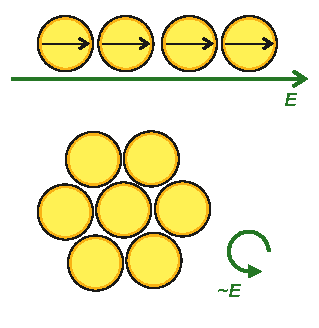
\includegraphics[width=0.5\textwidth]{Управляемое взаимодействие направленное поле}
\caption{Частицы расположенные сверху, находятся в стационарном внешнем электрическом поле, что делает их взаимодействие анизотропным. Частицы расположенные снизу, находятся в вращающимся  внешнем электрическом поле, что делает их взаимодействие изотропным.}
\label{risPolar}
\end{center}
\end{figure}

При наложении внешнего поля на коллоидную систему, частица поляризуется и потенциал взаимодействия выглядит следующим образом \cite{gel7}:
\begin{equation}
\varphi(\mathbf{r})=-\mathbf{E}_{0} \cdot \mathbf{r}+\sum_{\alpha} \int_{\Gamma^{\alpha}} \mathrm{d} S \sigma^{\alpha}\left(\mathbf{r}_{k}\right) G\left(\mathbf{r}, \mathbf{r}_{k}^{\alpha}\right),
\end{equation}
где $r_{k}^{\alpha} \in \Gamma^\alpha, \Gamma^\alpha$ - поверхность $\alpha$-ой частицы, $G\left(\mathbf{r}, \mathbf{r}_{k}^{\alpha}\right)$ - функция Грина в уравнении Лапласа, и суммирование проводится по всем частицам.

Данное уравнение решается численными методами, и при усреднении по углу позволяет довольно точно описывать коллоидные частицы во внешних электрических полях.

Это позволяет использовать коллоидные системы как модельные, для изучения свойств мягкой материи на уровне отдельных частиц. 

\section{Модельные потенциалы взаимодействий}

Для изучения влияния микроскопических свойств системы на макроскопические, используется так называемый метод \textbf{молекулярной динамики (МД)}, который заключается в численном моделировании системы, состоящей из достаточно большого количества частиц, по статистике которых можно судить о макроскопических свойствах. 

Данные моделирования заключаются в численном решение уравнений Ньютона для каждой отдельной частицы. Одним из преимуществ такого подхода является возможность создания систем с совершенно любыми потенциалами взаимодействия между частицами. Он позволяет моделировать эффекты разрушения, пластичность, температурное изменение свойств материала, фазовые переходы.

Одним из наиболее популярных модельных потенциалов взаимодействия частиц в таких системах, является потенциал Леннарда - Джонса:
\begin{equation}
U\left(R_{i j}\right)=\varepsilon\left[\left(\frac{R_{0}}{R_{i j}}\right)^{12}-2\left(\frac{R_{0}}{R_{i j}}\right)^{6}\right]=4 \varepsilon\left[\left(\frac{\sigma}{R_{i j}}\right)^{12}-\left(\frac{\sigma}{R_{i j}}\right)^{6}\right], 
\label{eqFullLJ}
\end{equation}
где $\varepsilon$ и $R_0$ - глубина потенциальной ямы и равновесное расстояние между частицами; $R_0 = 2^{1/6}\sigma$.

В то время как зависимость $R^{-6}$ получена теоретически и обусловлена силами Ван-дер-Ваальса, зависимость $R^{-12}$ выбрана из соображений удобства.

\begin{figure}[h]
\begin{center}
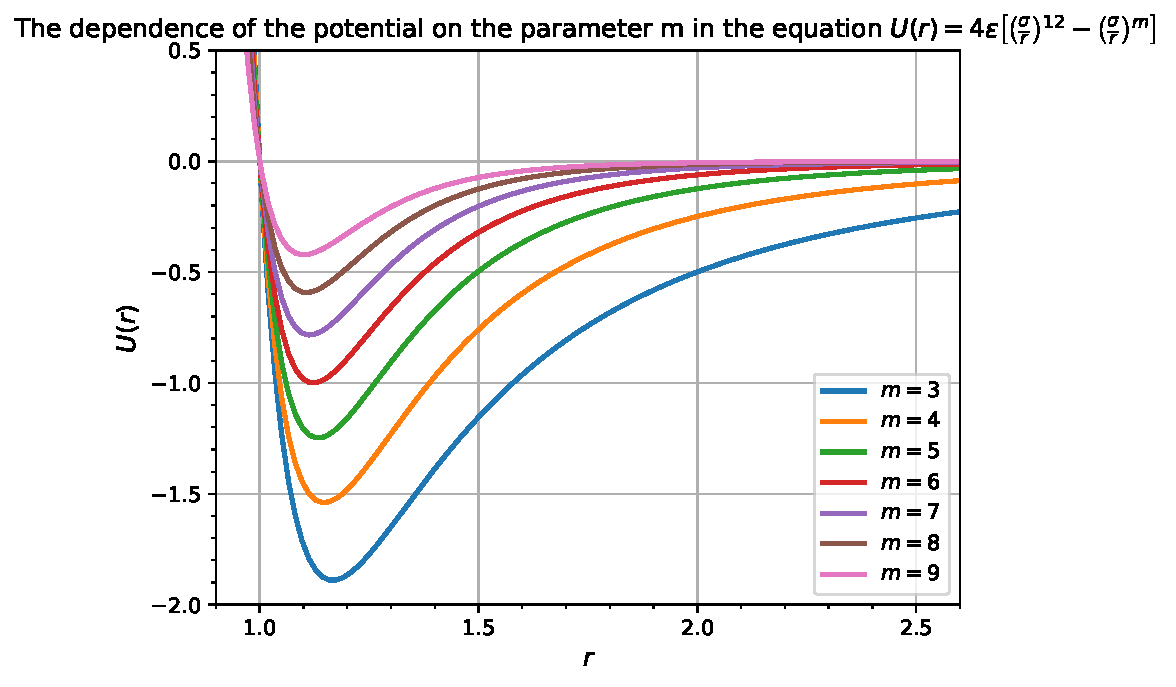
\includegraphics[width=\textwidth]{LJ}
\caption{Демонстрация обобщенного потенциала Леннарда--Джонса с различными степенями слагаемого, отвечающего за притяжение. $m = 6$ соответствует стандартному потенциалу Леннарда--Джонса.}
\label{risLJvar}
\end{center}
\end{figure}

Потенциал Леннарда--Джонса является простейшим из всех видов потенциалов у которого потенциальная энергия зависит от модуля расстояния между частицами. Несмотря на сильно ограниченные возможности в количестве макроскопических параметров, из-за наличия всего двух варьируемых параметров, потенциал весьма точно описывает свойства ряда веществ (прежде всего, кристаллических инертных газов), а также достаточно точно описывает силы взаимодействия \\ Ван--дер--Ваальса, играющие важную роль в твердых телах. К достоинству потенциала Леннарда--Джонса относится так же его вычислительная простота, не требующая вычисления иррациональных и трансцендентных функций.

Во многие модельных системах, такие как коллоидные суспензии и пылевые плазмы, парные взаимодействия на коротких расстояниях в основном описываются отталкиванием Юкавы \cite{phase59}.

Система точечных частиц в 2D геометрии, взаимодействует через попарно отталкивающий потенциал вида:
\begin{equation}
\varphi(r)=\frac{\varepsilon \lambda}{r} \exp \left(-\frac{r}{\lambda}\right)
\end{equation}

где $\varepsilon, \lambda$ - энергетические и экранирующие масштабы длин взаимодействия. Для заряженных частиц, погруженных в плазмоподобную экранирующую среду, энергетическая шкала равна:
\begin{equation}
\varepsilon=Q^{2} / 4 \pi \epsilon_{0} \lambda
\end{equation}

где $Q$ - заряд, $\epsilon_{0}$ - диэлектрическая проницаемость пространства.

Свойства систем Юкавы определяются двумя параметрами: параметром связи и параметром отбора. Первый определяется так:
\begin{equation}
\text{Г}=Q^{2} / 4 \pi \epsilon_{0} a k_{\mathrm{B}} T
\end{equation}

где $k_b$ - постоянная Больцмана, T - температура, $a=(\pi n)^{-1 / 2}$ - радиус Вигнера-Зейтца, где n - концентрация частиц на единицу объема.

Второй параметр равен:
\begin{equation}\kappa=a / \lambda\end{equation}

Заметим, что параметр связи - отношение потенциальной энергии взаимодействия двух соседних частиц к их кинетической энергии. Обычно говорят, что система находится в сильно связанном состоянии, когда это соотношение велико \cite{phase59}.

Различные физические величины в данных моделированниях удобно выражать через константы моделирования. В случае Леннарда-Джонса это  $\sigma, \varepsilon, m$, где $m$ - масса частиц, $\sigma$ - расстояние, на котором энергия взаимодействия становится равным нулю, $\varepsilon$ - глубина потенциальной ямы.

Метод молекулярной динамики, в данной работе, позволяет выяснить влияние дальнодействия притяжения на термодинамические свойства системы и параметры переноса.

\section{Цели и задачи бакалаврской работы}

\textbf{Цель работы} --
установить связь между дальнодействием притяжения в двумерной системе частиц, взаимодействующих посредством обобщенного потенциала Леннарда-Джонса, c фазовой диаграммой, и параметрами переноса.

\textbf{Задачи работы:}
\begin{enumerate}
\item Разработка программного комплекса для расчета явлений переноса в $2D$ системах.
\item Разработка методов определения термодинамических свойств системы по распределениям плотностей. 
\item Усовершенствование метода распознавание фаз и построения фазовых диаграмм.
\item Применение разработанных методов на различных потенциалах взаимодействия.
\item Применение наработок для изучения влияния потенциала взаимодействия на различные термодинамические параметры.
\end{enumerate}

\newpage
%\chapter*{Введение}
%\addcontentsline{toc}{chapter}{Введение}

\newpage
\begin{center}
\textbf{\large ГЛАВА 2 \\ Влияние дальнодействия притяжения на фазовые диаграммы}
\end{center}
\refstepcounter{chapter}


% \section*{}
\addcontentsline{toc}{chapter}{ГЛАВА 2. Влияние дальнодействия притяжения на фазовые диаграммы}

\section{Метод построения фазовых диаграмм с помощью разбиения на ячейки Вороного}\label{C2_1}

Для исследования многих термодинамических параметров системы, требуется знать принадлежность частиц к той или иной фазе (жидкой, твердой, газообразной, сверхкритической). Эту задачу решают некоторые алгоритмы классификации, которые используют априори известные положения всех частиц в системе для определения принадлежности к тому или иному классу. Например, проблема идентификации кластеров были рассмотрены в работах \cite{phase45} и \cite{phase46}, где данная проблема решается с помощью порогов для межчастичных расстояний и полной энергии частиц. Однако данные методы обладают существенными недостатками связанными с слишком грубой оценкой границ кластера, в первом случае, и требованием знания точного значения потенциала взаимодействия и всех скоростей частиц.

Метод исследования многочастичных систем с помощью диаграмм Вороного, рассмотренный в статье \cite{Ovcharov2017}, основан на триангуляции Делоне и разбиении систем частиц на ячейки Вороного. Данный метод позволяет разбить систему на области, по статистике которых можно судить о термодинамический параметрах данной системы, и фазовом составе.

Построив гистограмму Вороного для множества точек, каждой точке можно сопоставить ряд параметров:
\begin{itemize}
\item Площадь и плотность.
\item Число соседей (далее будет использован термин \textbf{соседняя частица}).
\item Параметр порядка и т.д.
\end{itemize}

Это позволяет использовать данный метод для изучения равновесного и неравновесного плавления кристаллов \cite{phase16, phase49, phase54, phase50, phase51, phase51, phase53}, парных корреляций \cite{phase55, phase59, phase56, phase57, phase58}, деформаций и дислокаций \cite{phase16, phase60}.

Под плотностью частицы имеется ввиду величина, обратная площади ячейки вороного, которой эта частица принадлежит:
\begin{equation}
\rho_i = 1 / S_i,
\label{eqRho}
\end{equation}
где $\rho_i$ - плотность соответствующей частицы, $S_i$ - ее площадь, определяема как площадь соответствующей ячейки.

Под \textbf{соседней частицей}, понимается частица, с которой имеется общее ребро у ячеек.

\begin{figure}[h]
\begin{center}
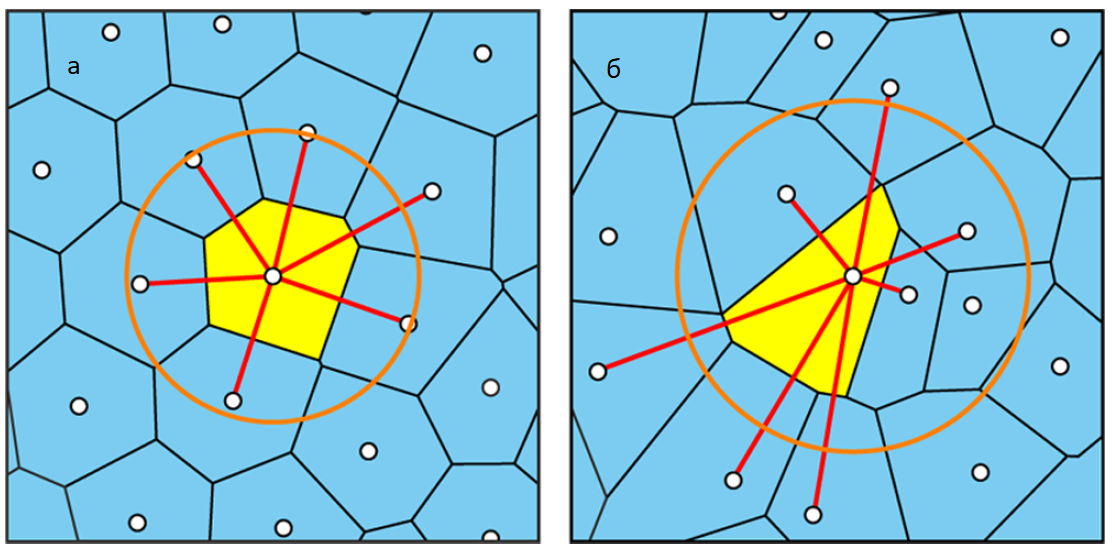
\includegraphics[width=0.7\textwidth]{rgcell}
\caption{Пример разбиения на ячейки Вороного в конденсированном кластере (а) и газе (б). Частицы представлены белыми точками, а ячейки, соответствующие рассматриваемым частицам раскрашены в желтый цвет. Радиус окружностей соответствует среднему расстоянию между частицей и ее соседями. Изображение взято из статьи \cite{Ovcharov2017}.}
\label{risFlucMed}
\end{center}
\end{figure}

На рисунке \ref{risFlucMed} показана часть $2D$ - системы, полученной с использованием МД-моделирования потенциала Леннарда-Джонса (LJ12-6) при плотности системы $\rho_0 = 0.4$.
Сравнивая ячейки Вороного в конденсированной среде и газе, можно заметить, что конденсированное состояние отличается меньшей площадью частиц, вследствие чего, частицы конденсата обладают большей плотностью, и соответственно, расположение частиц сильно ограниченно в пространстве, что ведет к более упорядоченной структуре и более правильной форме ячеек Вороного.

Это дает возможность ввести некоторую величину, которая показывает отклонение ячейки от правильной формы:
\begin{equation}
	R_{0i} = \sqrt{\frac{\pi}{2 S_i N_{ni}^2} \sum\limits_{i<k}^{N_{ni}} (r_{ij} - r_{ik})^2}, r_{ij} = |r_i - r_j|,
\end{equation}
где $S_i$ - площадь рассматриваемой частицы, $N_{ni}$ - количество соседей частицы, $r_{ij}$ - расстояние от рассматриваемой частицы до соседней.
Для уменьшения сильных колебаний величины $R_{0i}$, она усредняется по соседним частицам:
\begin{equation}\label{eqIrreg}
R_i = \frac{1}{N_{ni} + 1} \left( R_{0i} + \sum\limits_{j=1}^{N_{ni}} R_{0j} \right),
\end{equation}

Данная величина позволяет оценить среднеквадратичное смещение между соседними частицами, и нормировать их на площадь ячеек.
Далее она будет называться \textbf{параметром иррегулярности $R$}.

Этот параметр может найти применение не только в классификации частиц на фазы, но и для изучения плавления и горения веществ \cite{phase54}.

\begin{figure}[h]
\begin{center}
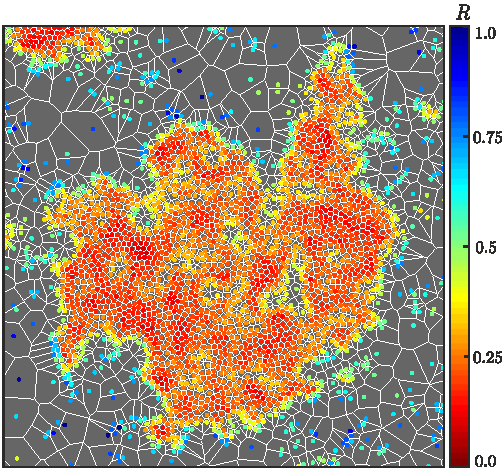
\includegraphics[width=0.7\textwidth]{MPI-Figure1}
\caption{Пример конденсированного кластера в системе с потенциалом Леннарда-Джонса. Ячейки вороного раскрашены в белый цвет, частицы раскрашены по величине параметра иррегулярности $R$. Изображение взято из статьи \cite{Ovcharov2017}.}
\label{risIrreg}
\end{center}
\end{figure}

На рисунке \ref{risIrreg} представлен конденсированный кластер, частицы которого раскрашены в соответствии с параметром иррегулярности. Чем он меньше, тем более упорядочена система. В идеальном кристалле данный параметр равен нулю.

Поскольку параметр $R$ мал для частиц, принадлежащих кластерам конденсата, мы можем использовать следующее неравенство для их определения:
\begin{equation}
R < R_t,
\end{equation}
где $R_t$ - порог параметра иррегулярности, ниже которого можно считать частицу конденсатом.

\begin{figure}[h]
\begin{center}
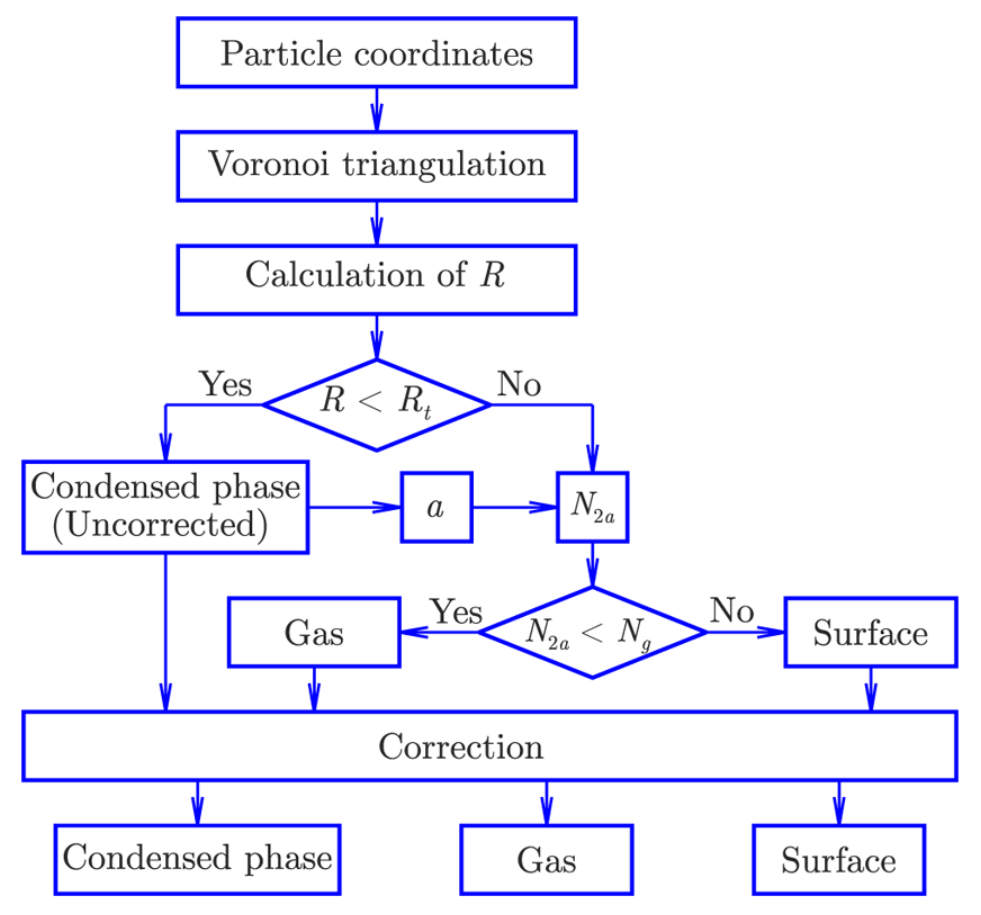
\includegraphics[width=0.5\textwidth]{shem_class}
\caption{Полная схема классификации частиц в системе. Изображение взято из статьи \cite{Ovcharov2017}.}
\label{risShemClass}
\end{center}
\end{figure}

Полная схема классификации частиц в системе, которая использует только координаты, представлена на рисунке \ref{risShemClass},
где $a$ - среднее расстояние между частицами; $N_g$ - некоторое пороговое значение для газовых частиц, находящихся на расстоянии $2a$ от выбранной частицы; $N_{2a}$ - число частиц, находящихся на расстоянии менее $2a$ от выбранной частицы. Если выполняется условие $N_{2a} < N_{g}$, то частица распознается как газ.
В данной работе константы приняты равными $R = 0.5, N_g = 5$.

По причине больших флуктуаций величины $R$, кроме обрезки по параметру $R_t$ и дополнительных условий требуется корректировка фаз.

Корректировка фаз включает в себя следующие условия:
\begin{itemize}
\item частица конденсата, не имеющая среди своих соседей частиц того же типа, является поверхностью.
\item частица конденсата, которая имеет среди соседних частиц, газовую частицу, является поверхностью.
\item газовая частица, не имеющая соседних частиц того же класса,  является поверхностью.
\item частица поверхности, все соседи которой принадлежат к классу "конденсат" или "газ", так же принадлежат к этому классу.
\end{itemize}
Система частиц прогоняется через эти условия несколько раз. Было установлено, что пяти раз достаточно для приемлемого результата классификации.

\begin{figure}[h]
\begin{center}
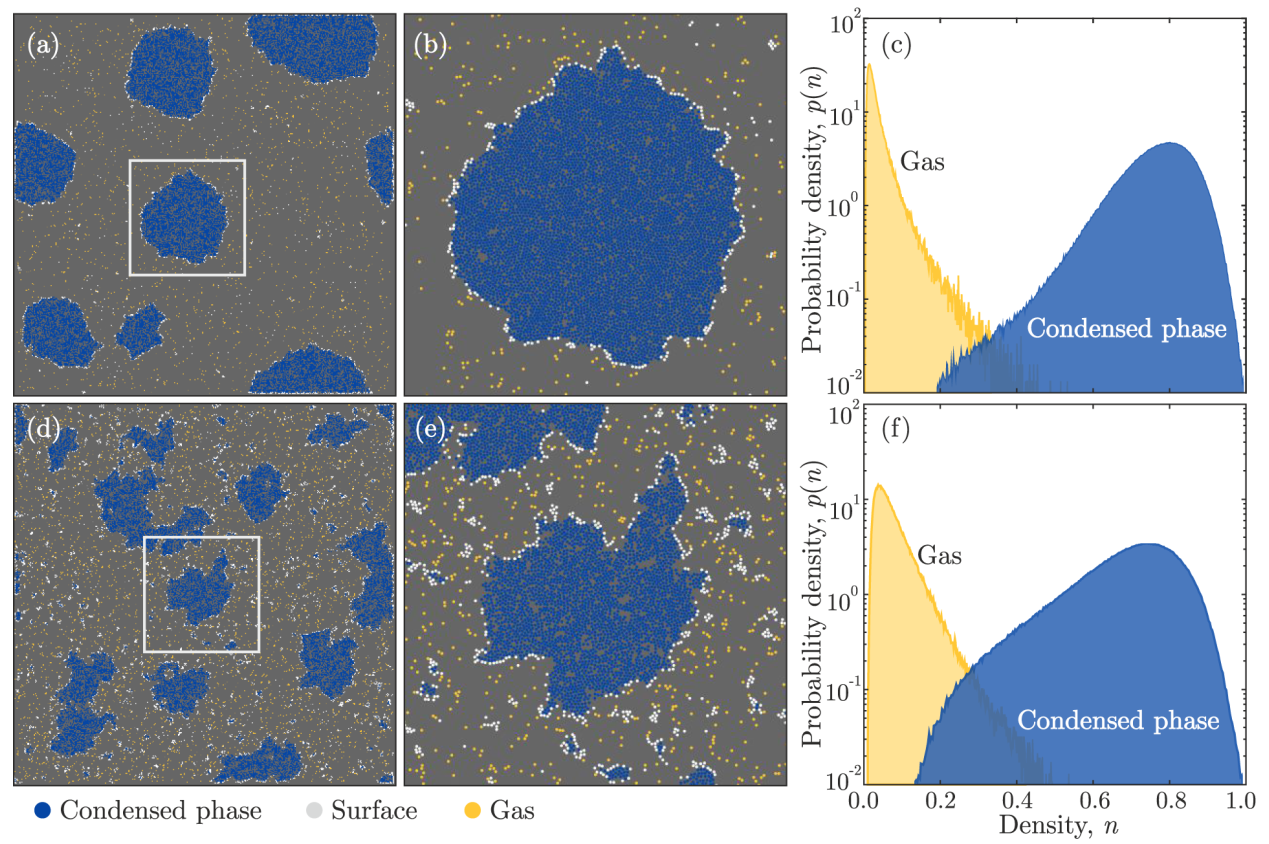
\includegraphics[width=0.8\textwidth]{articlePhaseAndDensity}
\caption{Слева - результат работы алгоритма, представленного на рисунке \ref{risShemClass}. Частицы разделены на 3 класса различными цветами: конденсат - синий, поверхность - белый, газ - желтый. Справа - плотность вероятности нахождения частицы газа и конденсата с данной плотностью. Изображение взято из статьи \cite{Ovcharov2017}.}
\label{risClassification}
\end{center}
\end{figure}

На рисунке \ref{risClassification} представлен результат классификации частиц данным методом в системе, описанной выше.
Однако у данного алгоритма есть ряд недостатков. Так например возможны случаи распознавания пустот с газом внутри конденсированного кластера, как его часть, а также наблюдаются крупные скопления частиц поверхности, внутри который нет частиц распознанных как конденсат.

После классификации всех частиц в системе на всех кадрах моделирования и расчета их плотностей по формуле \ref{eqRho}, возможно рассчитать математическое ожидание плотности конденсированных частиц и газа по-отдельности при данной температуре.
Повторив эти вычисления при различных температурах, можно построить фазовую диаграмму в координатах $\rho, T$.

Однако такой расчет плотности корректно работает только для конденсированных частиц, так как флуктуации размеров ячеек у конденсата невелики, и на их размер не оказывают влияния частицы газа и поверхности. На площадь же газовых частиц существенный эффект оказывают частицы поверхности, которые занимают сопоставимый с ними объем и тем самым увеличивают их плотность. Данная особенность является дефектом этого метода.

В рамках данной работы был существенно переработан алгоритм корректировки фаз, который помимо условий представленных в оригинальной работе включает дополнительные условия:
\begin{itemize}
\item частица поверхности, не имеющая среди соседей частиц газа, является конденсатом.
\item поверхностная частица, не имеющая среди соседей частиц конденсата, является газом.
\item частицы конденсата, плотность которых сопоставима с плотностью поверхностных частиц, являются поверхностью. Данная проверка делается дважды (перед всеми остальными и после).
\item частица конденсата, которая имеет меньше 3 соседних частиц, так же принадлежащих к конденсату, является поверхностью.
\end{itemize}
Эти условия позволяют отделить крупные пустоты внутри кристалла от самого кристалла, и определить крупные скопления поверхностных частиц как небольшие кластеры конденсата или газ.

Так же был переработан алгоритм вычисления плотности газа в системе. Плотность вычисляется косвенно, по формуле:
\begin{equation}
\rho_{gas} = \frac{N_{g}}{S - (N_{b} + N_{c}) / \mathbb{M}\rho_c},
\label{eqGas}
\end{equation}
где $S$ - суммарная площадь всех рассматриваемых кадров, $N_g, N_b, N_c$ - суммарное число частиц газа, поверхности и конденсата соответственно на всех рассматриваемых кадрах моделирования, $\mathbb{M}\rho_c$ - математическое ожидание плотности частиц конденсата на всех рассматриваемых кадрах.

При данном подходе, площадь поверхностных частиц считается равной плотности конденсата, что позволяет более объективно вычислять плотность газа в системе, и соответственно, более точно определять критические точки веществ, что будет рассмотрено в разделе \ref{C2_2}.

\section{Построение фазовых диаграмм для различных потенциалов взаимодействия}\label{C2_2}

В данной работе, для изучения влияния дальнодействия притяжения на фазовые диаграммы, были выбраны системы с обобщенным потенциалом взаимодействия Леннарда - Джонса (уравнение \ref{eqLJ}) с изменяющейся степенью слагаемого, отвечающего за притяжение:
\begin{equation}
U(r) = 4\varepsilon \left[ \left(\frac{\sigma}{r}\right)^{12} - \left(\frac{\sigma}{r}\right)^{m} \right],
\label{eqLJ}
\end{equation}
где $\varepsilon$ - константа, имеющая размерность энергии, $\sigma$ - константа, имеющая размерность длинны, $r$ - расстояние от центра частицы, $m$ - степень слагаемого, отвечающего за притяжение частиц, в данной работе исследуется ее влияние на фазовые диаграммы и параметры переноса. Далее будет использовано обозначение стандартного потенциала Леннарда - Джонса как LJ12-6, где 12 - степень отталкивания, 6 - степень притяжения.

В рамках данной работы были проведены моделирования для случаев $m = 3, 4, 5, 6, 7, 8, 9$ в программе LAMMPS, с параметрами, указанными в таблице \ref{tablParam}, где $\Delta T$ - шаг по температуре,  $\rho$ - плотность системы. Во всех численных экспериментах рассматривалась система в $NVT$ ансамбле, состоящая из 3600 частиц. В ходе моделирования было проделано 600000 итераций изменения системы, между которыми было $0.05\tau$ времени, где $\tau$ - безразмерное эффективное время. В процессе моделирования данные выводились в файл с периодом в 100 итераций расчета, всего, таким образом, было получено 6000 состояний системы с интервалом в $0.5\tau$ (далее эти состояния будут считаться кадрами моделирования). Что бы исключить эффекты, связанные с релаксацией системы, во всех моделированиях, в качестве данных для анализа, были взяты только последние 150 состояний, в которых система уже находится в равновесии.

Все потенциалы с различными степенями притяжения, рассмотренные в данной работе, изображены на рисунке \ref{risLJvar}.

Все величины, являются обезразмеренными на константы моделирования, такие как масса частиц, постоянная Больцмана, $\varepsilon$ и $\sigma$ в уравнении \ref{eqLJ} потенциала, равные единице.

\begin{table}[h]
\begin{center}
\begin{tabular}{| l | l | l | l | l | l | l | l |}
\hline
    & LJ12-3 & LJ12-4 & LJ12-5 & LJ12-6 & LJ12-7 & LJ12-8 & LJ12-9 \\ \hline
$m$   &    3    &     4   &    5    &    6   &  7   &  8    &   9  \\ \hline
$\Delta T$ & 0.06 & 0.03 & 0.02 & 0.02  & 0.003 & 0.003 & 0.002\\ \hline
$\rho_0$ & 0.3  &  0.4  &  0.4  &  0.4  &  0.4  &  0.4  &  0.4 \\ \hline
\end{tabular}
\end{center}
\caption{Параметры моделирования исследуемых систем. $m$ - степень слагаемого в уравнении \ref{eqLJ}, $\Delta T$ - шаг по температуре,  $\rho_0$ - плотность системы в целом, то есть количество частиц деленное на площадь всей рассматриваемой системы.}
\label{tablParam}
\end{table}

На примере потенциала Леннарда - Джонса (LJ12-6) продемонстрирована работа модифицированного алгоритма распознавания фаз при различной температуре.

\begin{figure}[h]
\begin{center}
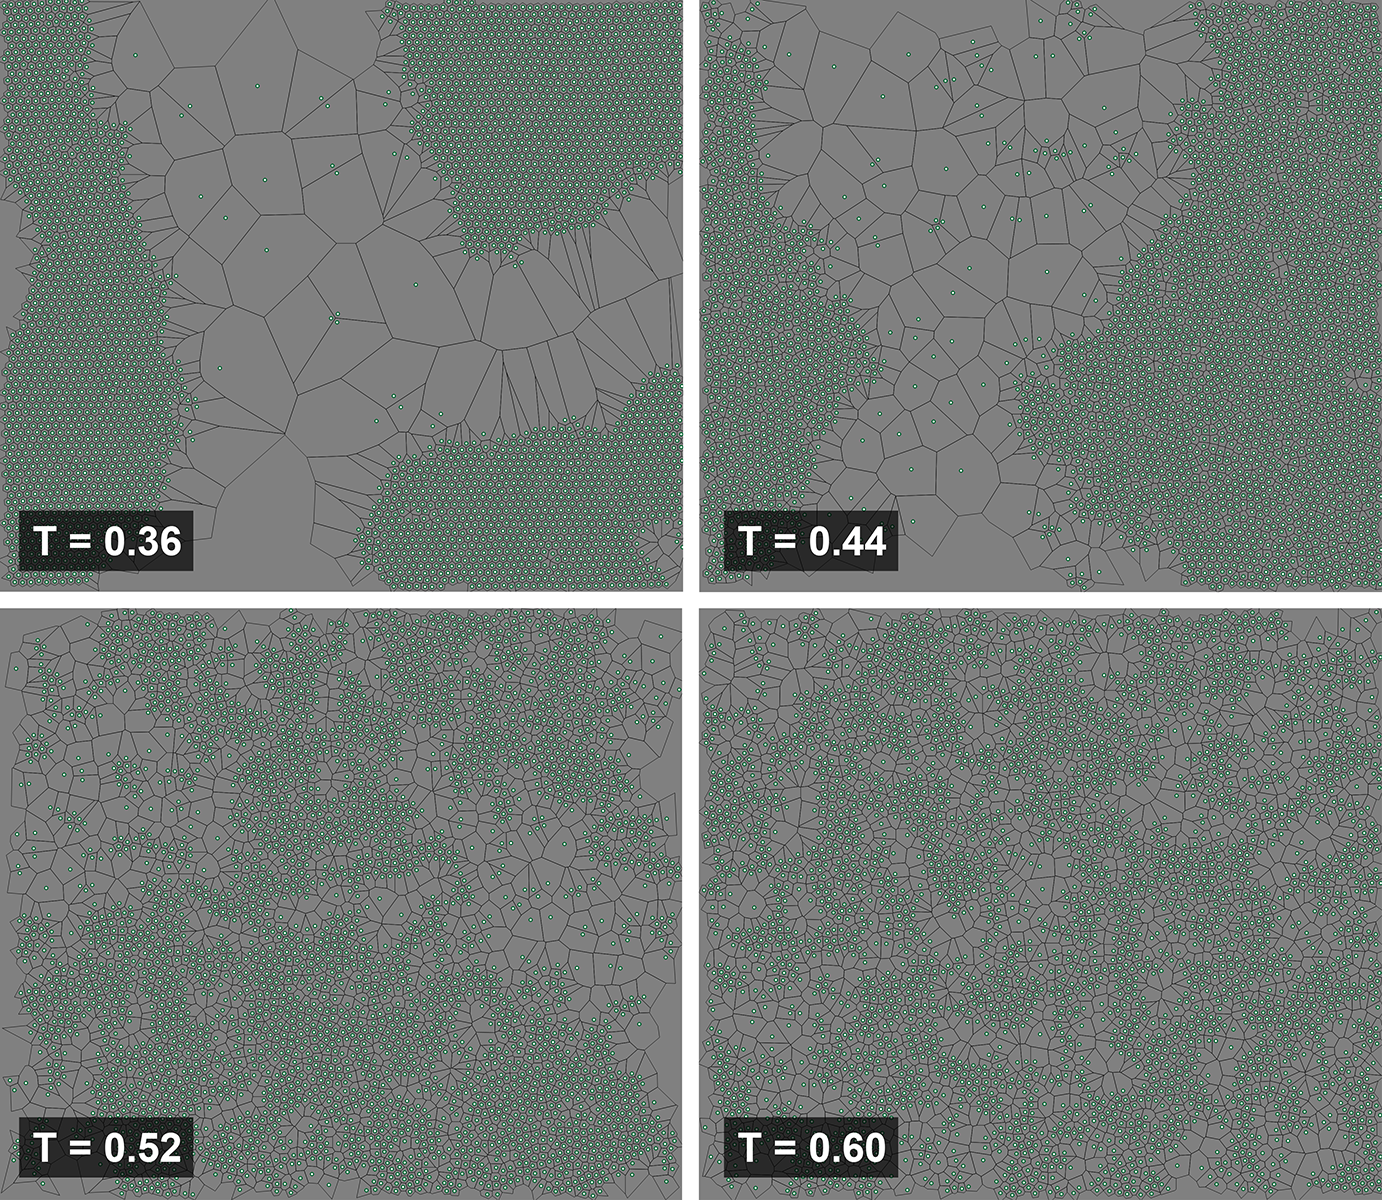
\includegraphics[width=0.7\textwidth]{Voronoi}
\caption{Разбиение на ячейки Вороного при различной температуре на примере стандартного потенциала Леннарда--Джонса.}
\label{risvoronoiExp}
\end{center}
\end{figure}

На рисунке \ref{risvoronoiExp} изображено разбиение системы на ячейки Вороного для различных температур. При $T = 0.36$ система находится в состоянии кристалла, при $T = 0.44$ в жидком. Также на рисунке представлена система, как выяснится далее, в критической точке ($T = 0.52$) и соответствующая максимальным флуктуациям плотности в системе ($T = 0.60$).

\begin{figure}[h]
\begin{center}
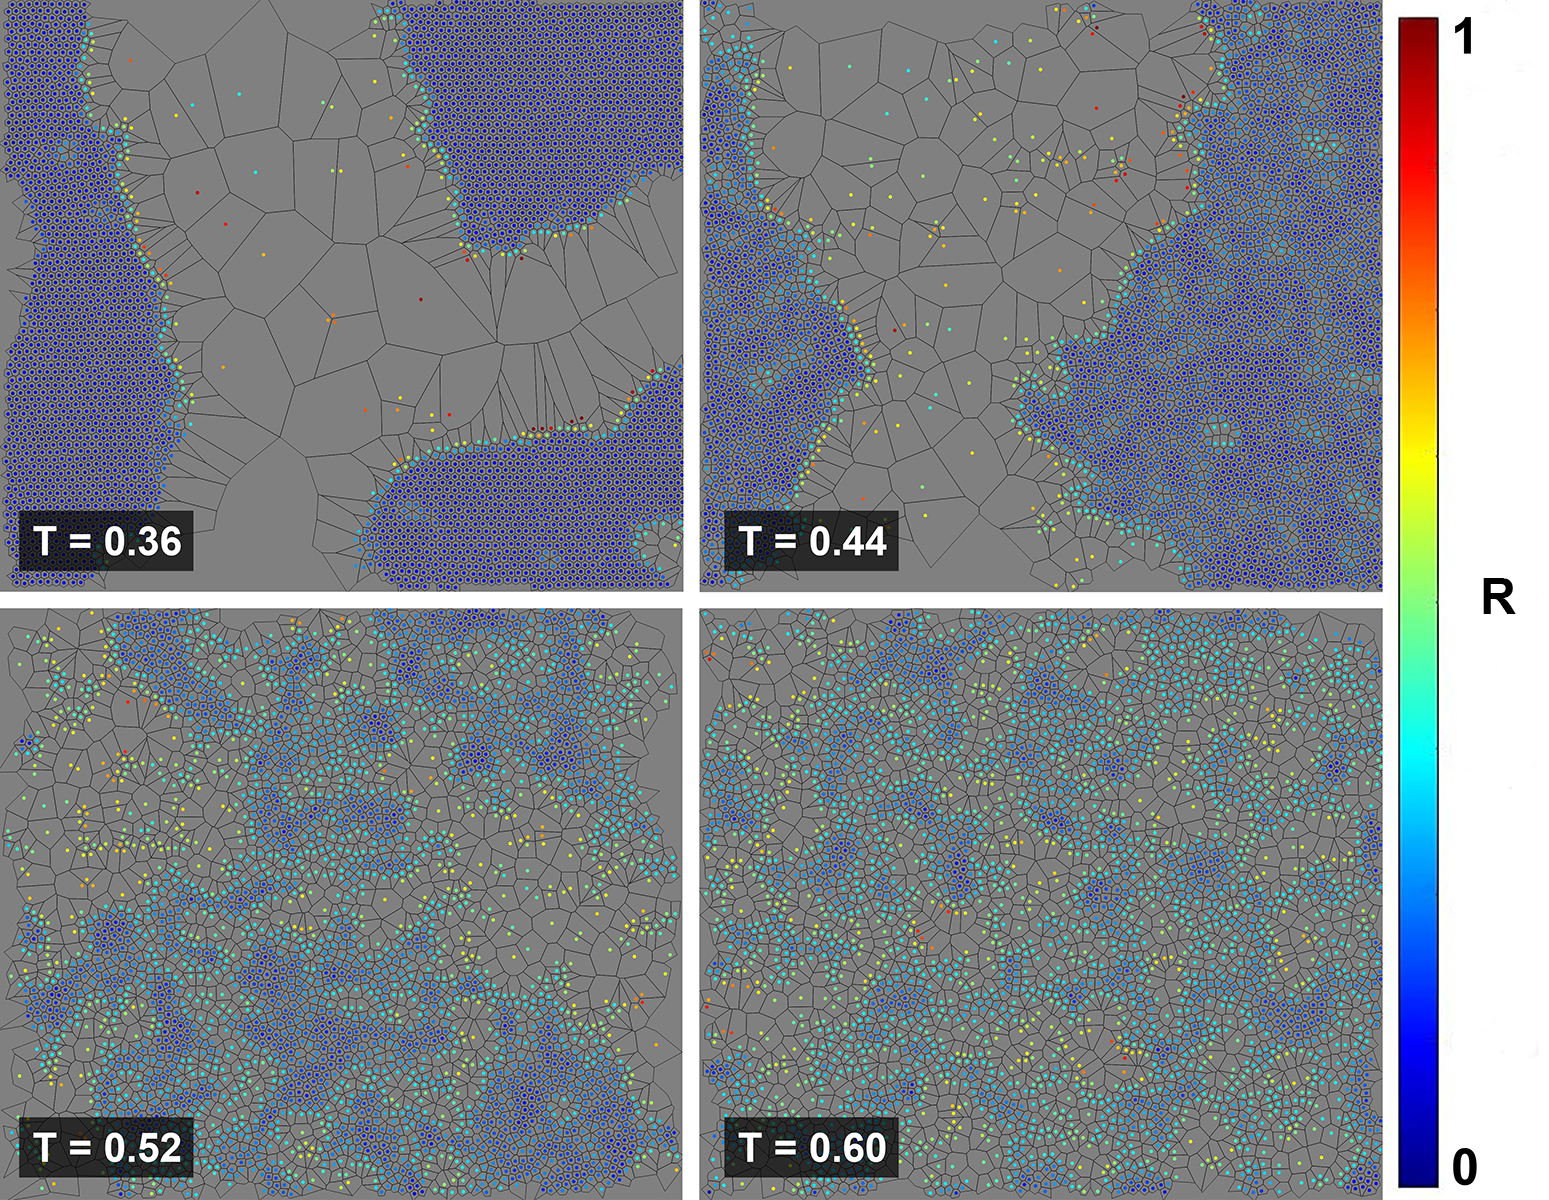
\includegraphics[width=0.7\textwidth]{RG}
\caption{Параметр иррегулярности $R$ в исследуемой системе, на примере потенциала взаимодействия Леннарда-Джонса при различной температуре.}
\label{risIregExp}
\end{center}
\end{figure}

\begin{figure}[h]
\begin{center}
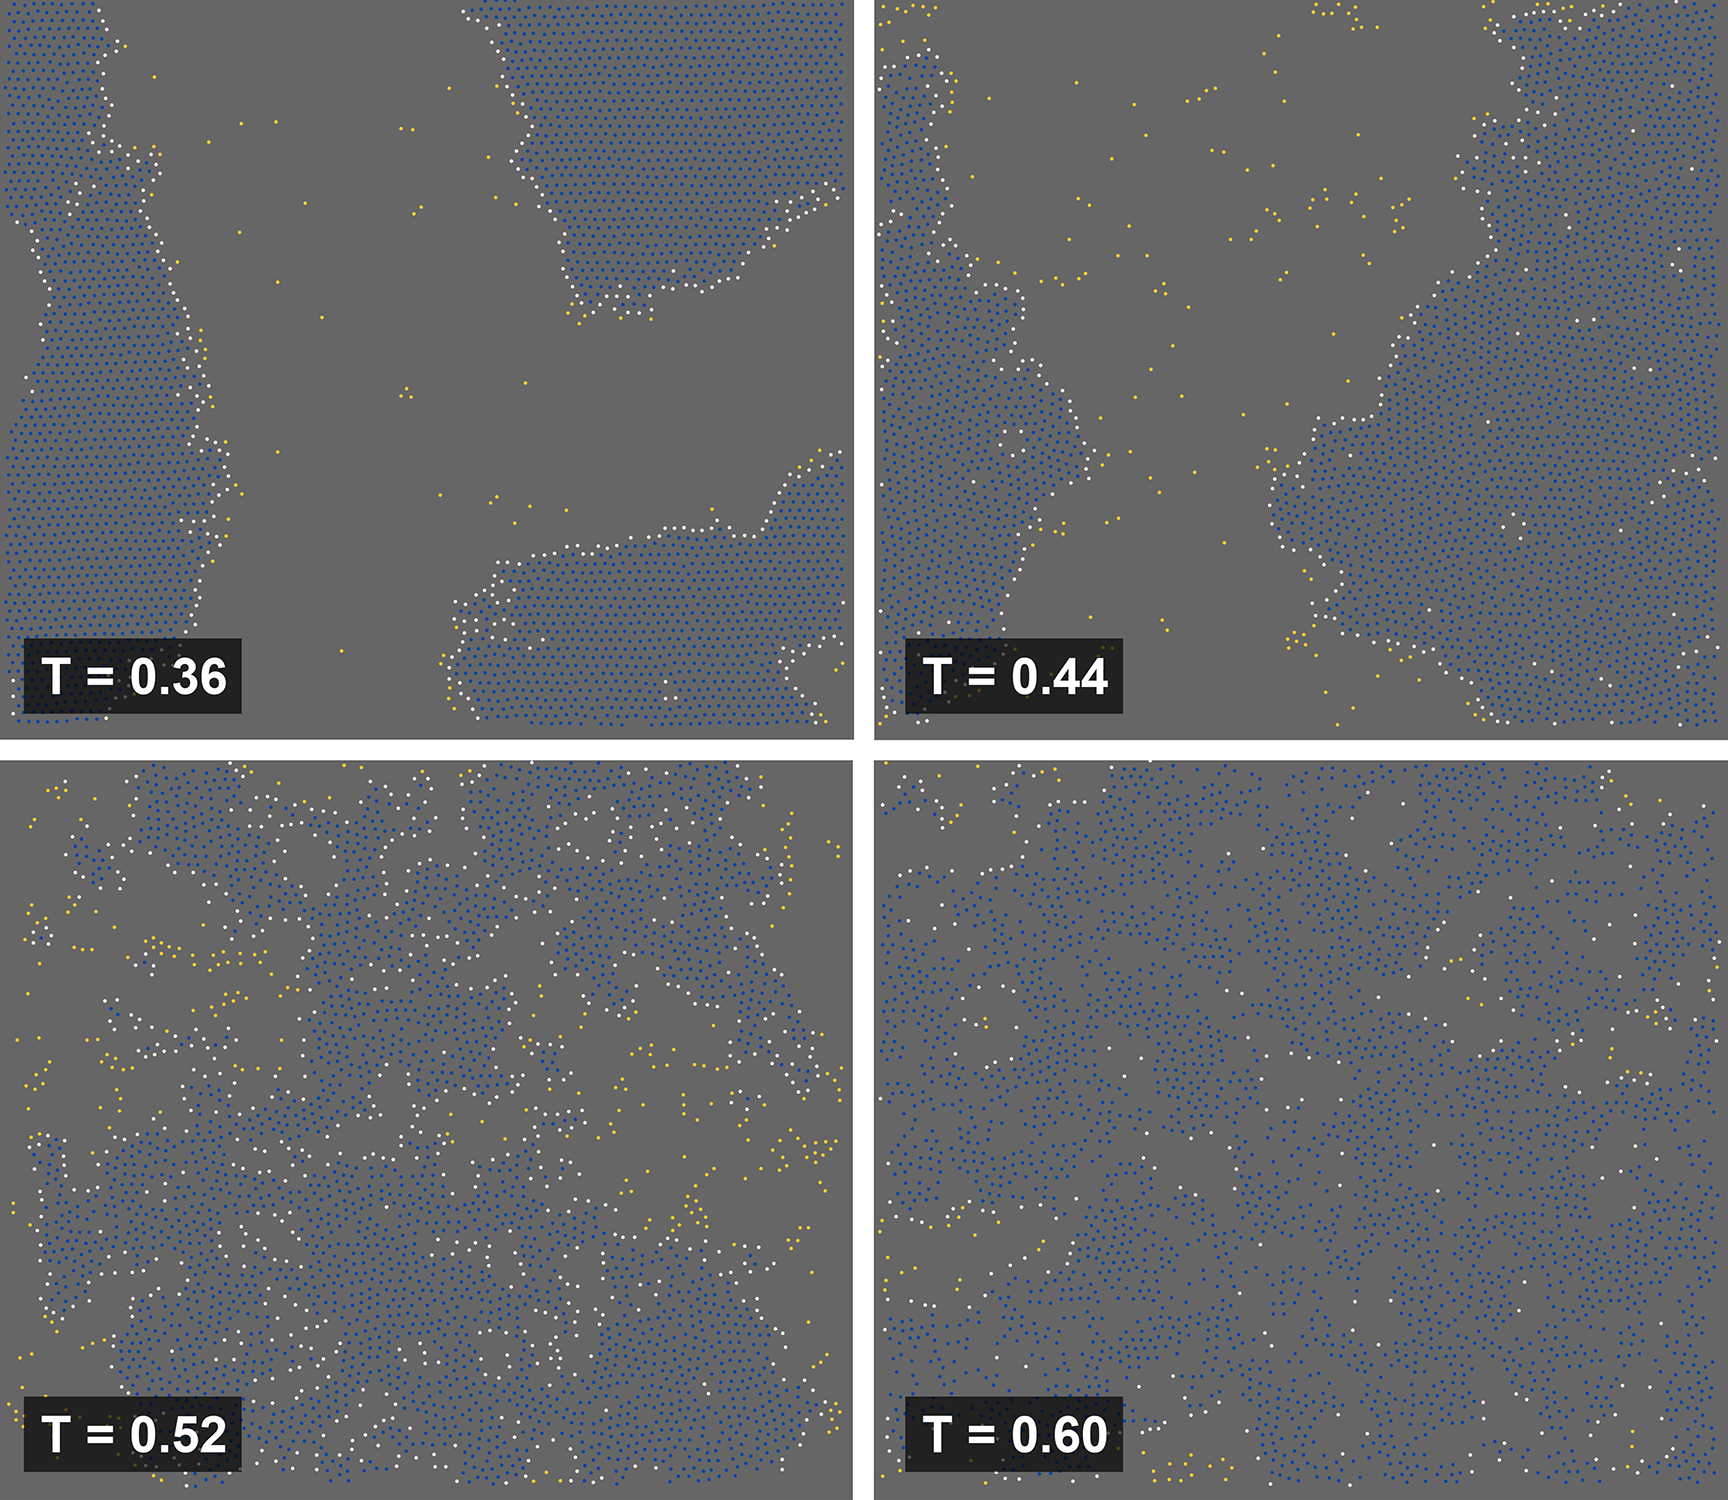
\includegraphics[width=0.7\textwidth]{classification}
\caption{Классификация частиц в исследуемой системе на примере стандартного потенциала Леннарда-Джонса при различной температуре.}
\label{risClassExp}
\end{center}
\end{figure}

После построения диаграммы Вороного проводится расчет параметра иррегулярности, представленного в разделе \ref{C2_1}. Результат расчета параметра изображен на рисунке \ref{risIregExp}. Затем, после корректировки фаз, получаем принадлежность каждой частицы к классу конденсата, газа или поверхности (рисунок \ref{risClassExp}).

Как можно увидеть на рисунке \ref{risClassExp}, данный метод лишен недостатков, описанных в главе \ref{C2_1}, связанных с распознаванием фаз.

\begin{figure}[h]
\begin{center}

\begin{minipage}[h]{0.45\linewidth}
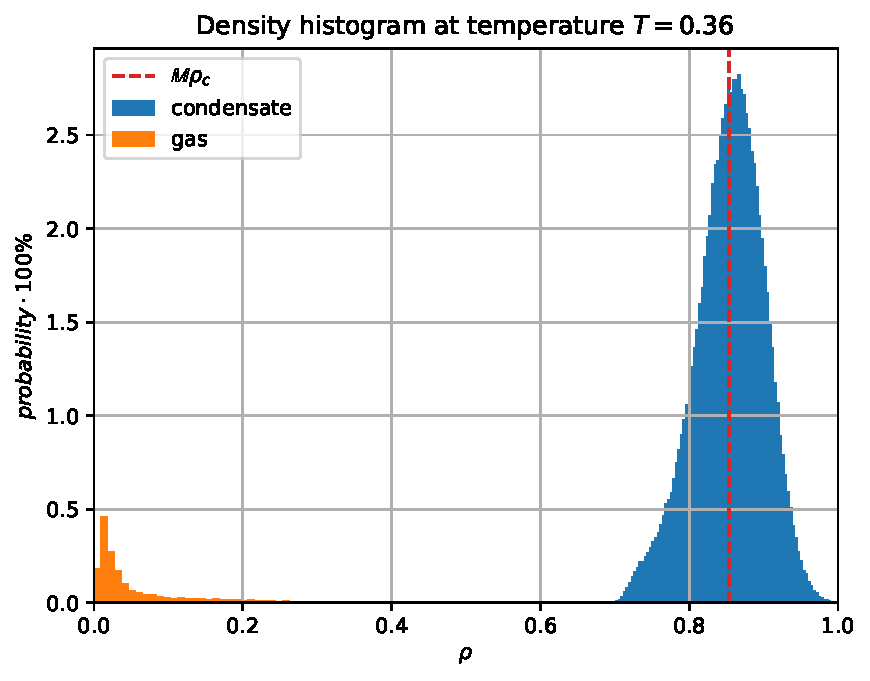
\includegraphics[width=\textwidth, keepaspectratio]{plot_hist_all_0.360}
\end{minipage}
%\hfill
\begin{minipage}[h]{0.45\linewidth}
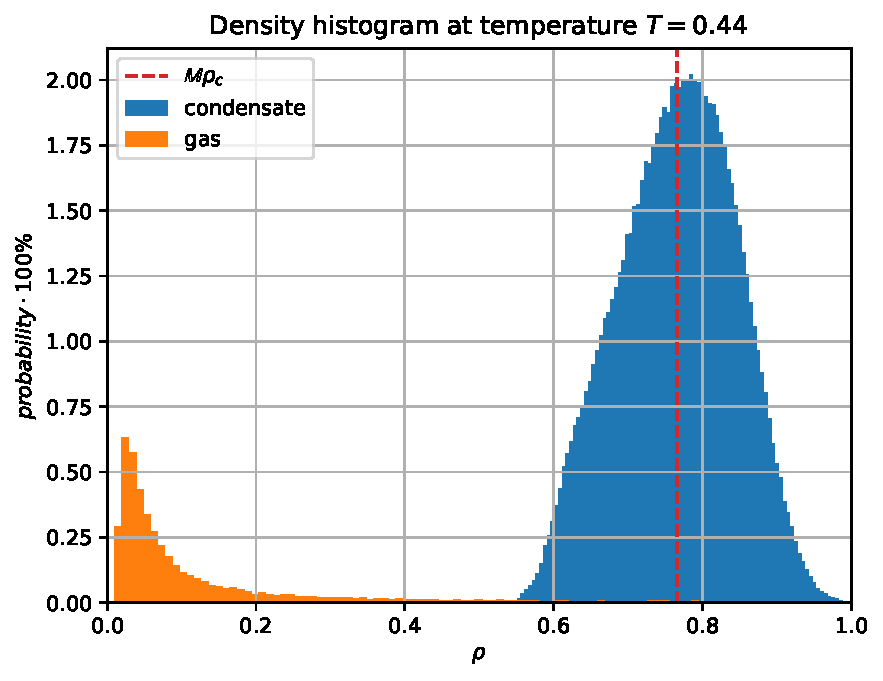
\includegraphics[width=\textwidth, keepaspectratio]{plot_hist_all_0.440}
\end{minipage}

\begin{minipage}[h]{0.45\linewidth}
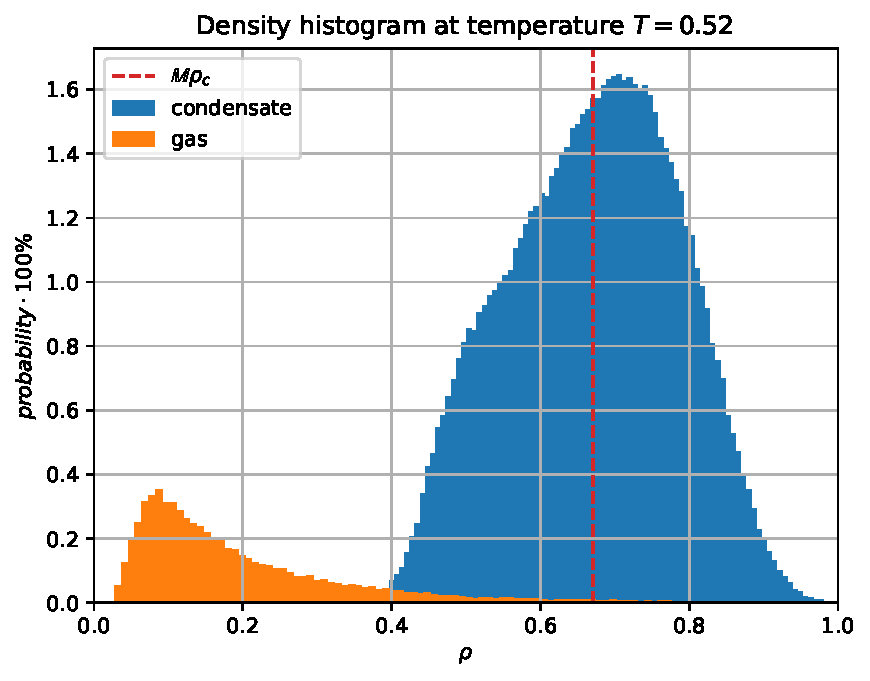
\includegraphics[width=\textwidth, keepaspectratio]{plot_hist_all_0.520}
\end{minipage}
%\hfill
\begin{minipage}[h]{0.45\linewidth}
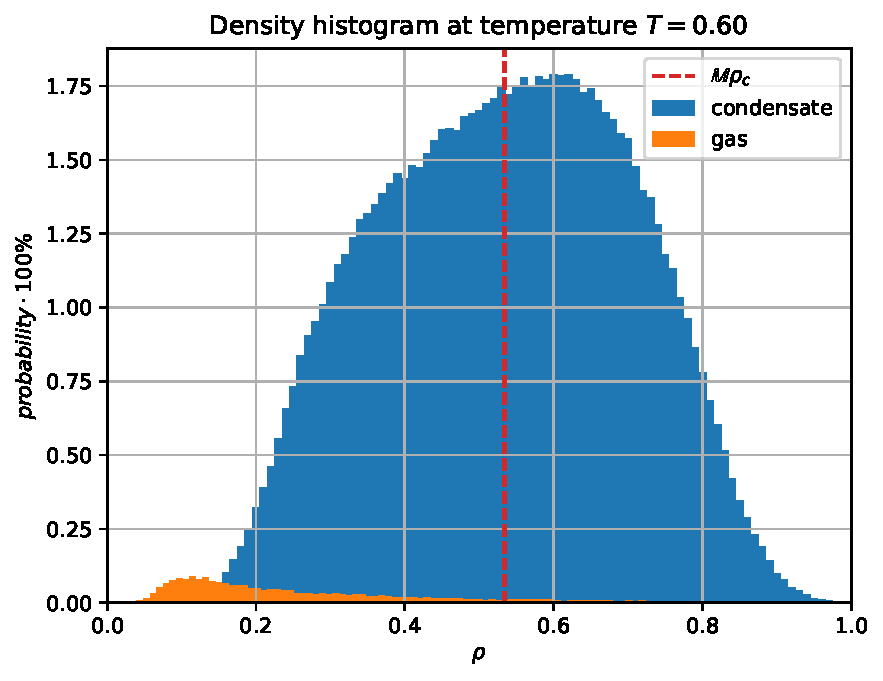
\includegraphics[width=\textwidth, keepaspectratio]{plot_hist_all_0.600}
\end{minipage}
\caption{Распределение плотностей частиц конденсата и газа при различных температурах. Синим цветом обозначен конденсат, оранжевым  - газ.}
\label{risRhoM}
\end{center}
\end{figure}

После классификации частиц, можно приступать к определению математического ожидания плотности газа и конденсата. На рисунке \ref{risRhoM} изображена график вероятности нахождения частицы в данной фазе с данной плотностью. Через значение плотности конденсата, указанное на рисунке красной пунктирной линией, можно по формуле \ref{eqGas} найти плотность газа в системе, и повторяя данную процедуру при различной температуре и значениях степени $m$, можно получить фазовые диаграммы для систем с различными потенциалами взаимодействия. Результаты построения фазовых диаграмм для исследуемых потенциалов изображены на рисунке \ref{risPhaseDiagrammExp}.

\begin{figure}[h]
\begin{center}
\begin{minipage}[h]{0.45\linewidth}
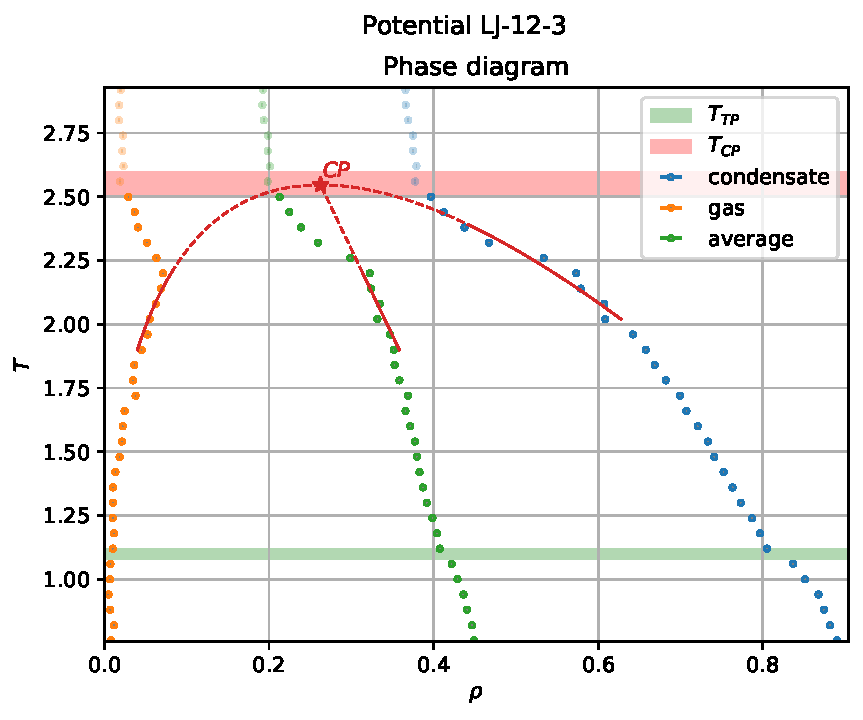
\includegraphics[width=\textwidth, keepaspectratio]{plot_phase_diagram_Potential LJ-12-3_1}
\end{minipage}
%\hfill
\begin{minipage}[h]{0.45\linewidth}
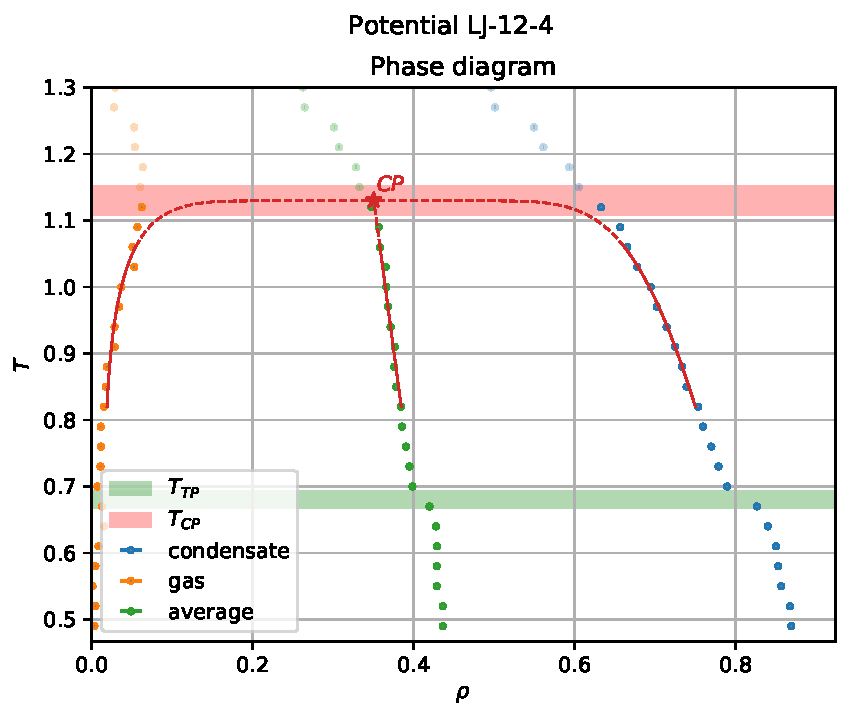
\includegraphics[width=\textwidth, keepaspectratio]{plot_phase_diagram_Potential LJ-12-4_1}
\end{minipage}

\begin{minipage}[h]{0.45\linewidth}
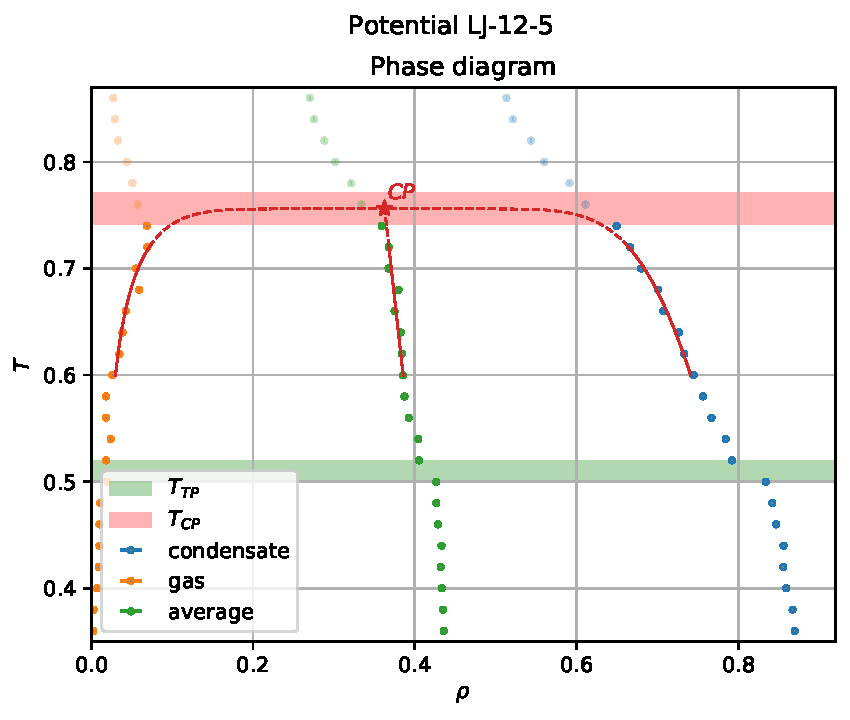
\includegraphics[width=\textwidth, keepaspectratio]{plot_phase_diagram_Potential LJ-12-5_1}
\end{minipage}
%\hfill
\begin{minipage}[h]{0.45\linewidth}
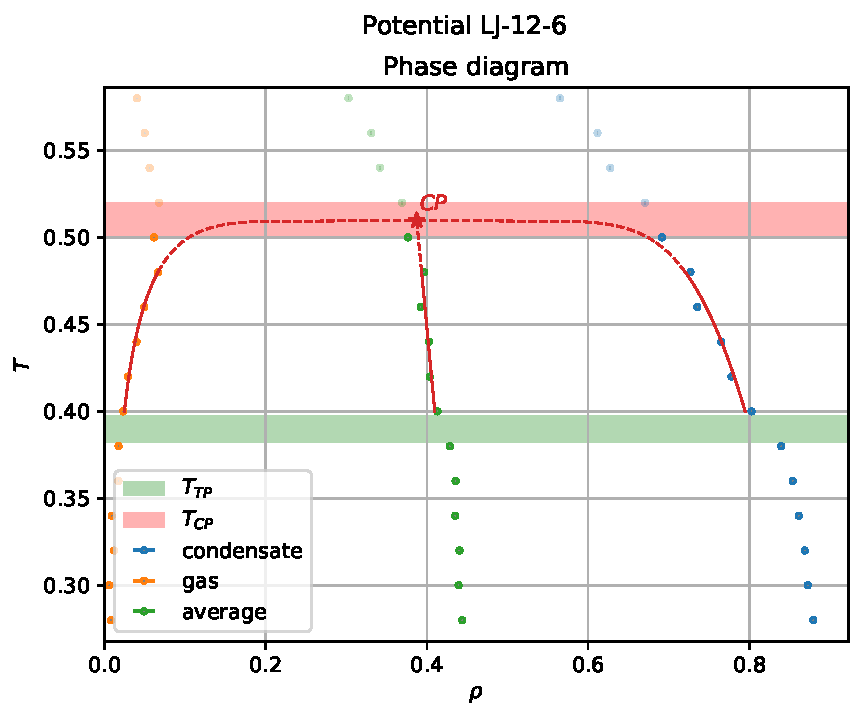
\includegraphics[width=\textwidth, keepaspectratio]{plot_phase_diagram_Potential LJ-12-6_1}
\end{minipage}
\caption{Фазовые диаграммы для систем с исследуемыми потенциалами взаимодействия. Подробности в основном тесте.}
\label{risPhaseDiagrammExp}
\end{center}
\end{figure}

Как известно \cite{fitPhase}, бинодали фазовых диаграммы в координатах $\rho, T$, вблизи критики, описываются следующими уравнениями:
\begin{equation}
\begin{aligned}
\rho_l - \rho_g &\simeq A (T_{CP} - T)^{\beta_c} \\
\frac{\rho_l + \rho_g}{2} &\simeq \rho_{CP} + a(T_{CP} - T)
\end{aligned}
\label{eqFitFhase}
\end{equation}
где $T_{CP}, \rho_{CP}$ - эффективная температура и плотность критической точки, $A, a$ - варьируемые параметры, $\rho_l, \rho_g$ - плотность жидкости и газа соответственно, $\beta_c$ - критический индекс системы.

Согласно источнику \cite{classCrit}, класс универсальности системы зависит от степени притяжения между частицами. Так, система LJ12-3 демонстрирует классическое поведение, для которого критический индекс $\beta_c = 1/2$, для всех остальных потенциалов, рассматриваемых в данной работе, $\beta_c = 1/8$.

Для более точного и удобного определения критической точки с помощью аппроксимации бинодалей, можно записать систему уравнений \ref{eqFitFhase} в следующем виде:
\begin{equation}
f_g(T) = \frac{T-a}{b} - A(T_{CP} - T)^{\beta_c}
\label{eqFitFhaseGas}
\end{equation}
\begin{equation}
f_l(T) = \frac{T-a}{b} + A(T_{CP} - T)^{\beta_c}
\label{eqFitFhaseLicuid}
\end{equation}
\begin{equation}
f_a(T) = \frac{T-a}{b},
\label{eqFitFhaseAverage}
\end{equation}

где уравнение \ref{eqFitFhaseGas} описывает газовую бинодаль, \ref{eqFitFhaseLicuid} - конденсированную, \ref{eqFitFhaseAverage} - их среднее значение, $A, a, b, T_{CP}$ - варьируемые параметры. 

Тогда можно составить функцию невязки, при минимизации которой получить наилучшую аппроксимацию бинодалей и значение критической температуры и плотности.

Условие наилучшей подгонки варьируемых параметров выглядит следующим образом:
\begin{equation}
\min \left(\sum\limits_{k} \left[ f_g(T_{g, k}) - n_{g, k}  \right]^2 + \sum\limits_{k} \left[ f_l(T_{l, k}) - n_{l, k}  \right]^2 + \sum\limits_{k} \left[ f_a(T_{g, k}) - n_{a, k}  \right]^2 \right),
\label{eqFitResidual}
\end{equation}
где суммирование производится по выбранным для аппроксимации точкам, а $n_g, n_l, n_a$ - соответствующие плотности выбранных точек. 

Точки могут быть выбраны не обязательно из одного температурного диапазона, для лучшей точности, чаще всего, выбирается немного различный диапазон. Это связано с некоторыми особенностями данного метода и бесконечным временем релаксации системы вблизи критической точки. Например при приближении к критической точке, из-за выравнивания плотности, существенно падает среднее значение параметра иррегулярности, из-за чего большинство частиц в системе начинает распознаваться как конденсат. В связи с этим, резко начинает падать плотность газа, что не соответствует действительности, поэтому газовая бинодаль аппроксимируется только до момента, пока не меняет свой знак вторая производная плотности по температуре. Данный эффект также влияет и на среднее значение газовой и конденсированной бинодали, поэтому среднее значение также аппроксимируется только до данной температуры.

Конденсированная же ветвь ведет себя более стабильно, и аппроксимация может проводиться по температурам чуть больше, чем для газа и среднего значения, однако в связи с бесконечным временем релаксации системы в критической точке, система не успевает отрелаксировать, и значение плотности конденсата вблизи критики становятся выше реального значения. Поэтому, при аппроксимации следует учитывать, что функция, аппроксимирующая конденсированную ветвь бинодали, должна проходить не выше самих точек.

Аппроксимация, проведенная данным методом, изображена на рисунке \ref{risPhaseDiagrammExp}, где красной цельной линией обозначен диапазон температур, точки из которого участвуют в аппроксимации, а красной штриховой - экстраполяция функций \ref{eqFitFhaseGas}, \ref{eqFitFhaseLicuid}, \ref{eqFitFhaseAverage} c найденными на предыдущем шаге подгоночными константами.

Как можно видеть, она довольно хорошо аппроксимирует точки фазовой диаграммы, что позволяет относительно точно определить критическую температуру и плотность системы.
Критические температуры и плотности, определенные данным способом, а также тройные точки систем, приведены в таблице \ref{tablSystemConst}.

\begin{table}[h]
\begin{center}
\begin{tabular}{| l | l | l | l | l | l | l | l |}
\hline
            & LJ12-3   & LJ12-4   & LJ12-5   & LJ12-6   & LJ12-7   & LJ12-8 & LJ12-9  \\ \hline
$T_{CP}$    & 2.54     &  1.13    &  0.76    &    0.51  & 0.38     & 0.26  & 0.18   \\ \hline
$T_{TP}$    & 1.1     & 0.68     & 0.51     & 0.40     & 0.31     & 0.23  & 0.16   \\ \hline
$\rho_{CP}$ & 0.26     &  0.35    &  0.36    &  0.39    & 0.39     & 0.42  & 0.43   \\ \hline
\end{tabular}
\end{center}
\caption{Параметры фазовых диаграмм для различных потенциалов взаимодействия. $T_{CP}$ - критическая температура, $\rho_{CP}$ - критическая плотность системы, $T_{TP}$ - температура тройной точки.}
\label{tablSystemConst}
\end{table}

Зная критические точки для потенциалов с различным притяжением, можно установить его роль в фазовой диаграмме вещества.

\section{Анализ гистограмм распределения}\label{C2_3}

Из источника \cite{Yur54} следует, что равновесные колебания вблизи среднего значения объема определяются уравнением состояния системы, и соответствующая функция распределения вероятности $p(V)$ равна:
\begin{equation}
p(V) \varpropto \exp\left[ \frac{1}{2T} \left( \frac{\partial P}{\partial V} \right)  \left(V - V_0 \right)^2 \right],
\label{eqPv}
\end{equation}
где $P$ - давление, $V_0$ - максимум распределения объема частиц (площади в $2D$ случае), $V$ - объем (площадь в $2D$ случае) частиц.
Тогда можно численно оценить производную $\frac{\partial P}{\partial V}$ и термодинамические величины через нее выражаемые.

Перепишем формулу \ref{eqPv} для колебаний плотности системы, сделав замену $V = 1 / \rho$, и получим следующее уравнение:
\begin{equation}
\begin{aligned}
p(\rho) &\varpropto \exp \left[ - K \left(\rho_{max}- \rho \right)^2 \right] \\
K &= \frac{1}{2T\rho_{max}^2} \left( \frac{\partial P}{\partial \rho} \right)
\end{aligned}
\label{eqFitRho}
\end{equation}
где $\rho_{max}$ - плотность максимума распределения.

\begin{figure}[htbp!]
\begin{center}
\begin{minipage}[h]{0.45\linewidth}
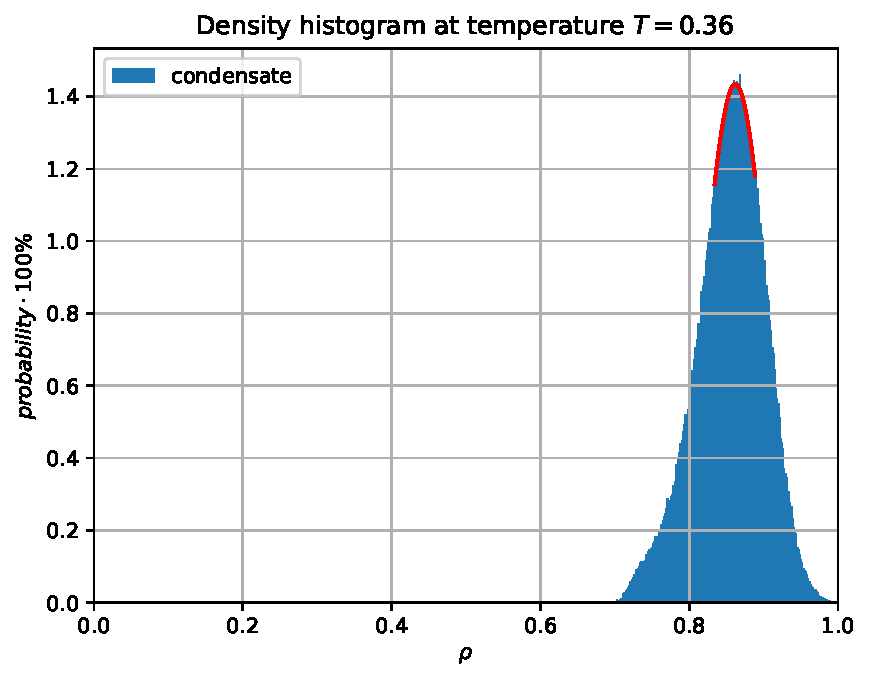
\includegraphics[width=\textwidth, keepaspectratio]{plot_hist_fit_0.360}
\end{minipage}
%\hfill
\begin{minipage}[h]{0.45\linewidth}
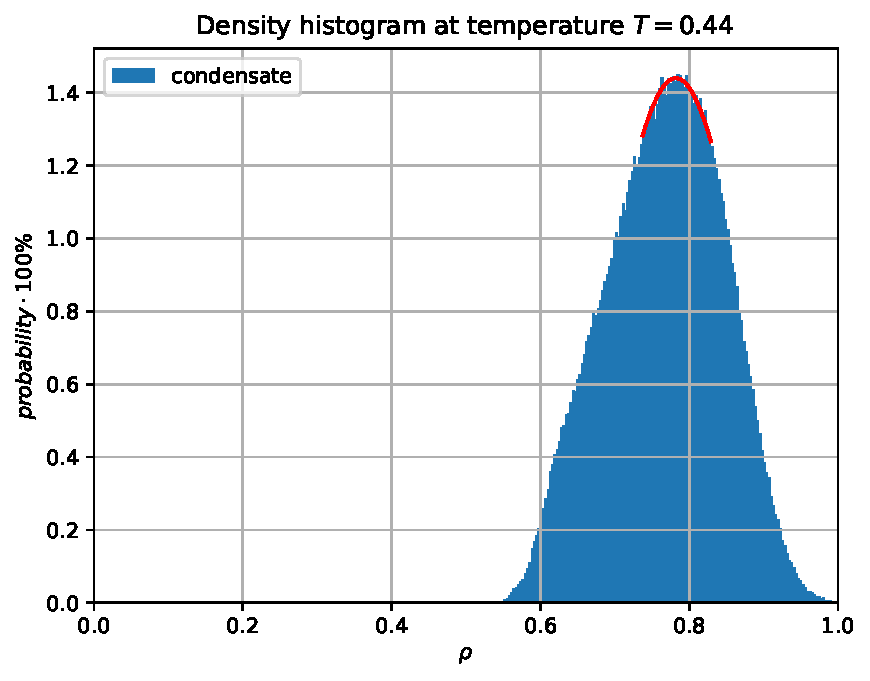
\includegraphics[width=\textwidth, keepaspectratio]{plot_hist_fit_0.440}
\end{minipage}

\begin{minipage}[h]{0.45\linewidth}
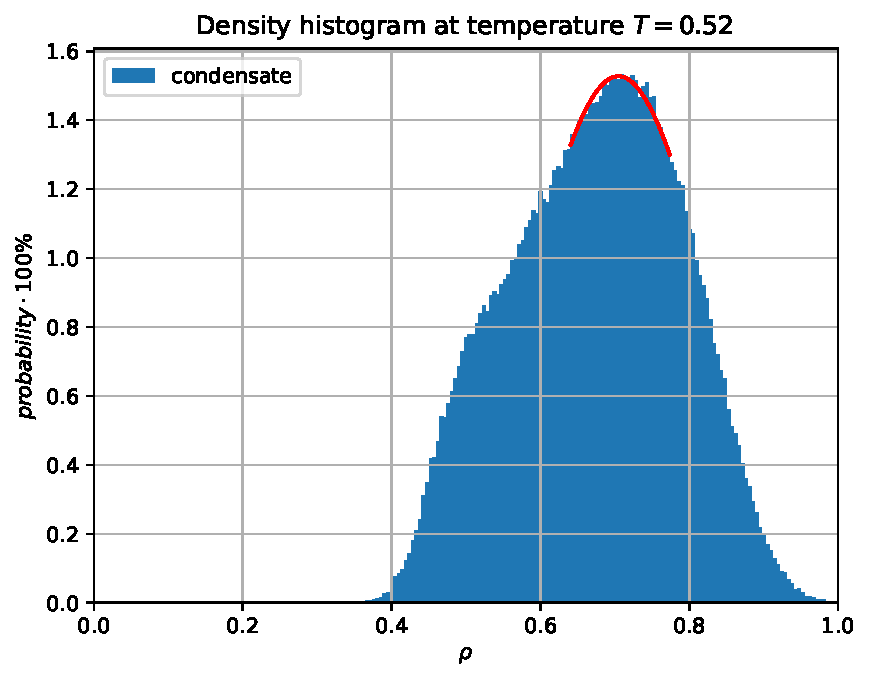
\includegraphics[width=\textwidth, keepaspectratio]{plot_hist_fit_0.520}
\end{minipage}
%\hfill
\begin{minipage}[h]{0.45\linewidth}
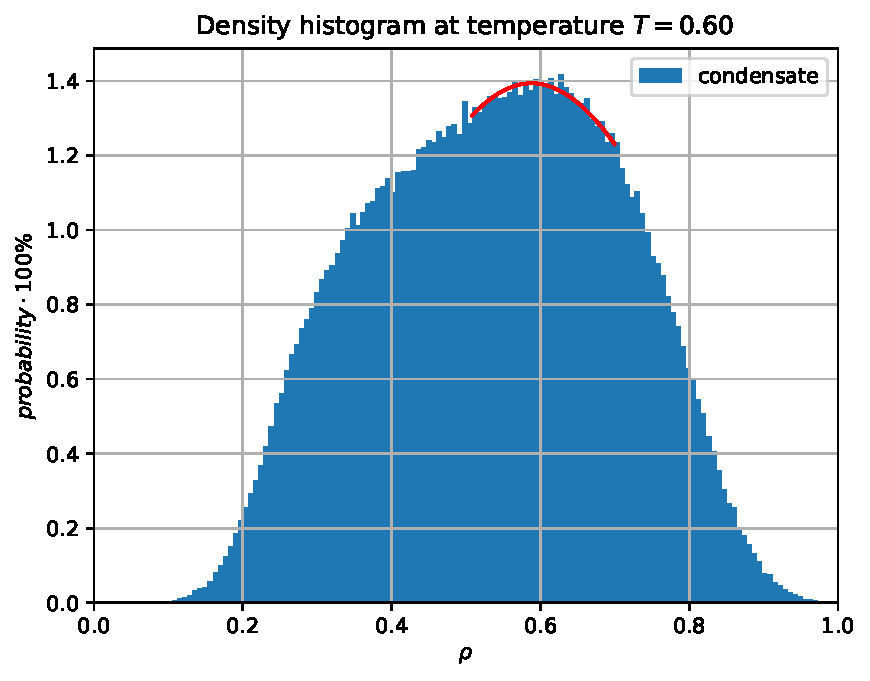
\includegraphics[width=\textwidth, keepaspectratio]{plot_hist_fit_0.600}
\end{minipage}
\caption{Аппроксимация пика распределения плотности при различной температуре.}
\label{risHistFit}
\end{center}
\end{figure}

При аппроксимации пика распределения плотности, возникают проблемы с автоматическим определением подгоняемых под уравнение \ref{eqFitRho} точек при различных температурах и величине статистики. Для решения этой проблемы, было решено брать точки, отстоящие от пика распределения на $k\sigma$, где $k$ - экспериментально определяемый коэффициент зависящий от формы распределений, для данных систем взятый равным 0.5, $\sigma$ - стандартное отклонение величины $\rho$ от среднего значения.  

Аппроксимируя данным способом верхушку распределения плотностей, для различных температур каждой системы (рисунок \ref{risHistFit}), получаем температурную зависимость коэффициента $K$, стоящего перед квадратичным слагаемом в разложении, представленную на рисунке \ref{risK}.

\begin{figure}[htbp!]
\begin{center}
\begin{minipage}[h]{0.45\linewidth}
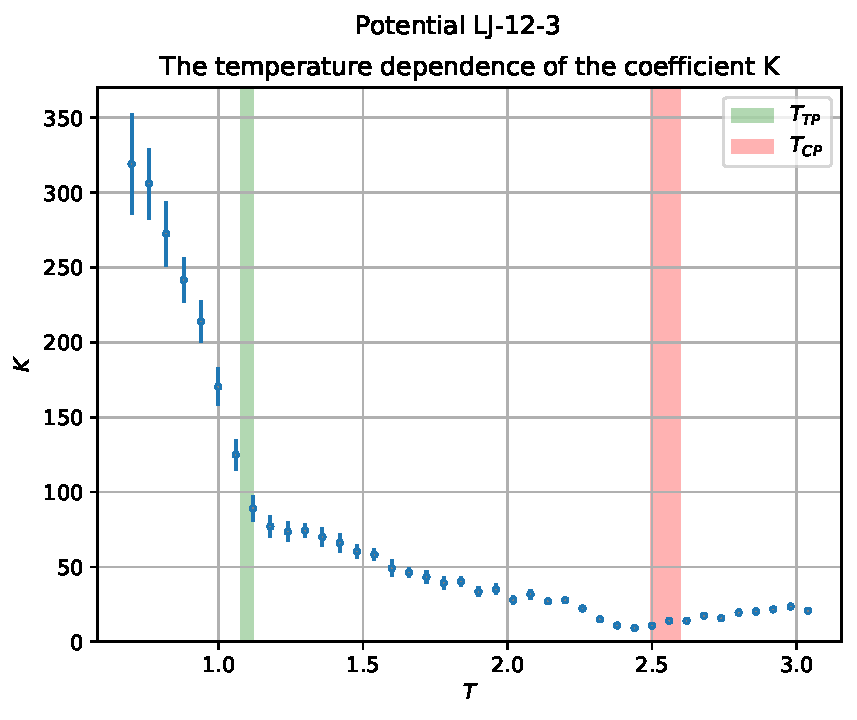
\includegraphics[width=\textwidth, keepaspectratio]{plot_K_Potential LJ-12-3_1}
\end{minipage}
%\hfill
\begin{minipage}[h]{0.45\linewidth}
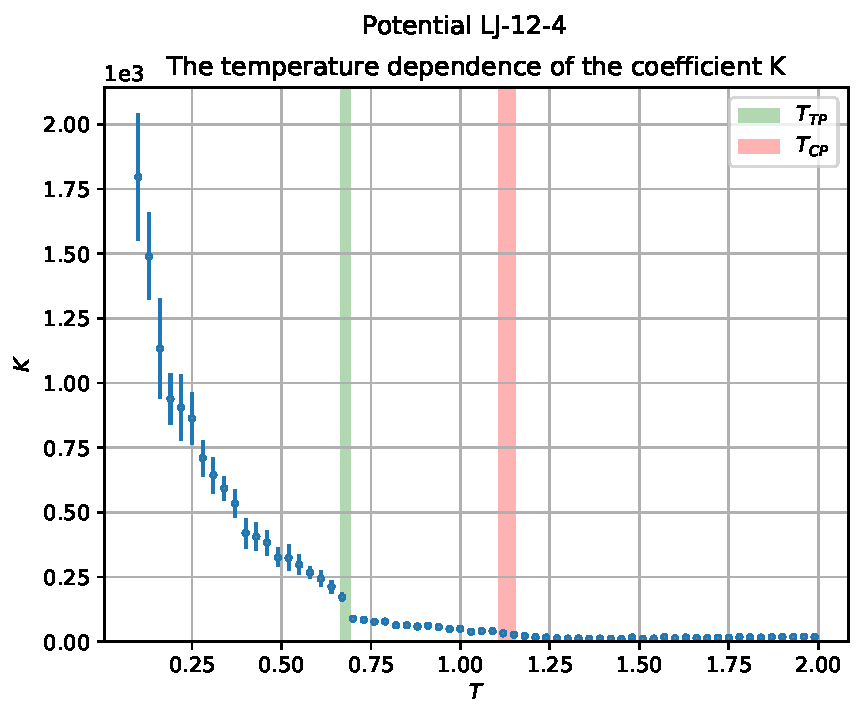
\includegraphics[width=\textwidth, keepaspectratio]{plot_K_Potential LJ-12-4_1}
\end{minipage}

\begin{minipage}[h]{0.45\linewidth}
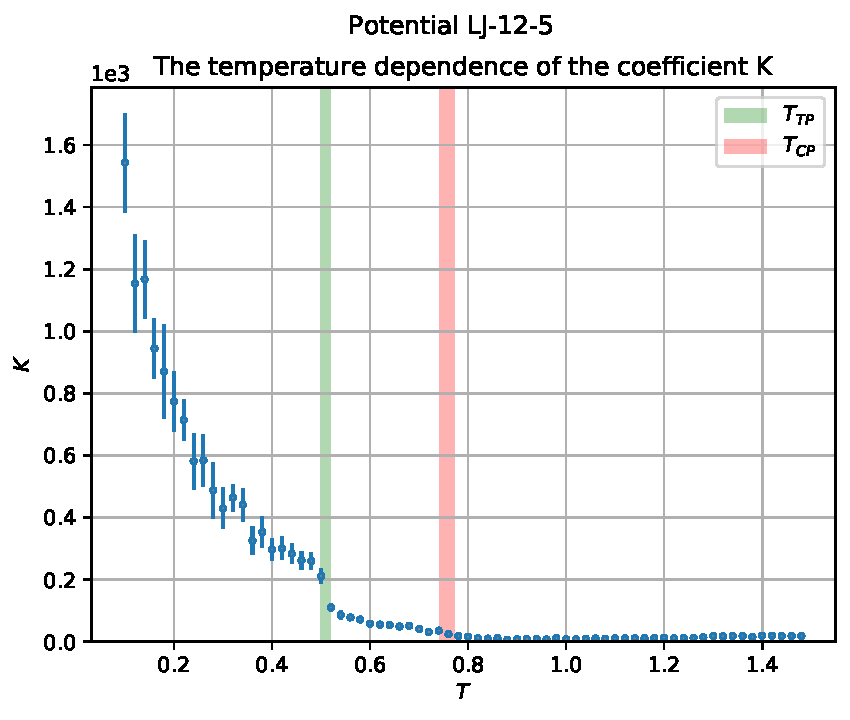
\includegraphics[width=\textwidth, keepaspectratio]{plot_K_Potential LJ-12-5_1}
\end{minipage}
%\hfill
\begin{minipage}[h]{0.45\linewidth}
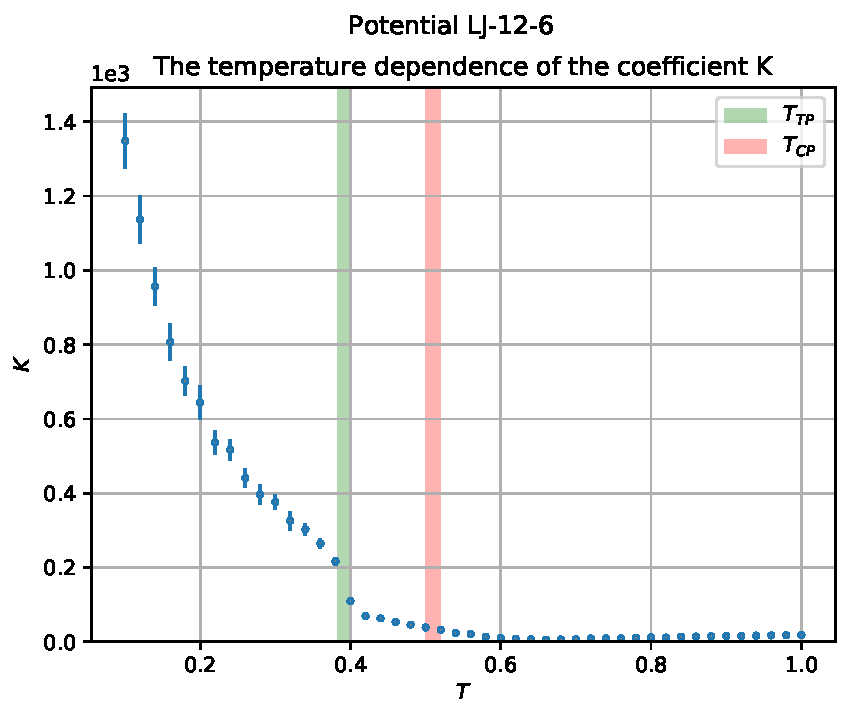
\includegraphics[width=\textwidth, keepaspectratio]{plot_K_Potential LJ-12-6_1}
\end{minipage}
\caption{Температурная зависимость коэффициента $K$.}
\label{risK}
\end{center}
\end{figure}

Через данный коэффициент можно выразить некоторые свойства системы, определяемые производной $\frac{\partial \rho}{\partial P}$, например сжимаемость вещества и адиабатическую скорость звука.

По определению, сжимаемость и адиабатическая скорость звука выражаются следующими формулами:
\begin{equation}
\beta = \frac{1}{\rho_0} \frac{\partial \rho}{\partial P}
\label{eqBetaClassic}
\end{equation}
\begin{equation}
C = \sqrt{\frac{\partial P}{\partial \rho}},
\label{eqCClassic}
\end{equation}
где $\beta$ - сжимаемости, $C$ - скорость звука в веществе.

Выразив данные величины через коэффициент $K$, получим следующие формулы:
\begin{equation}
\beta = \frac{1}{2T\rho_0\rho_{max}^2K}
\label{eqBeta}
\end{equation}
\begin{equation}
C = \rho_{max}\sqrt{2TK}
\label{eqC}
\end{equation}
Проведя вычисления при различных температурах, получаем зависимость сжимаемости и скорости звука в системе, рисунки \ref{risBeta} и \ref{risC}.

\begin{figure}[h]
\begin{center}
\begin{minipage}[h]{0.45\linewidth}
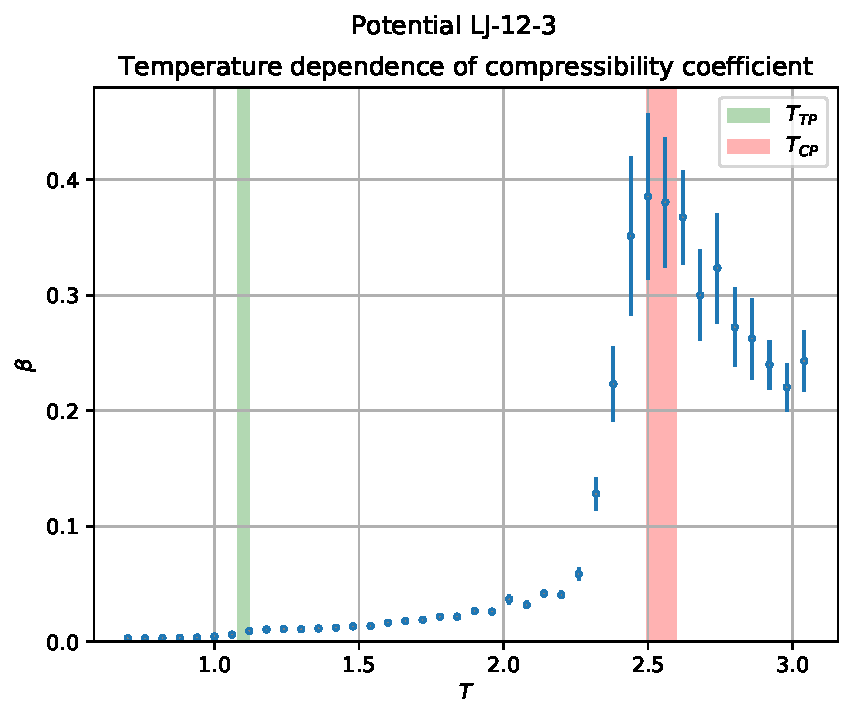
\includegraphics[width=\textwidth, keepaspectratio]{plot_compress_Potential LJ-12-3_1}
\end{minipage}
%\hfill
\begin{minipage}[h]{0.45\linewidth}
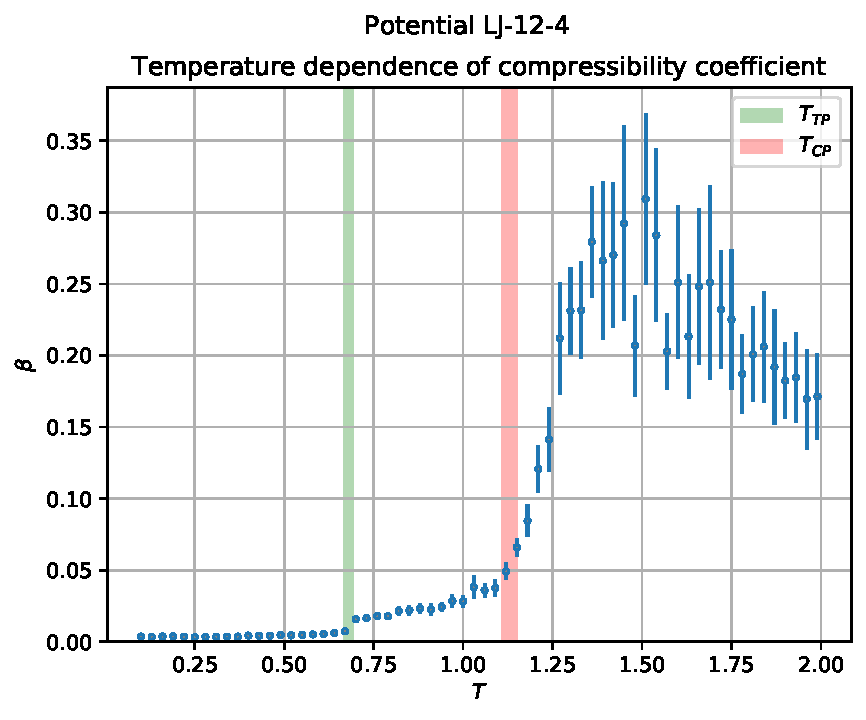
\includegraphics[width=\textwidth, keepaspectratio]{plot_compress_Potential LJ-12-4_1}
\end{minipage}

\begin{minipage}[h]{0.45\linewidth}
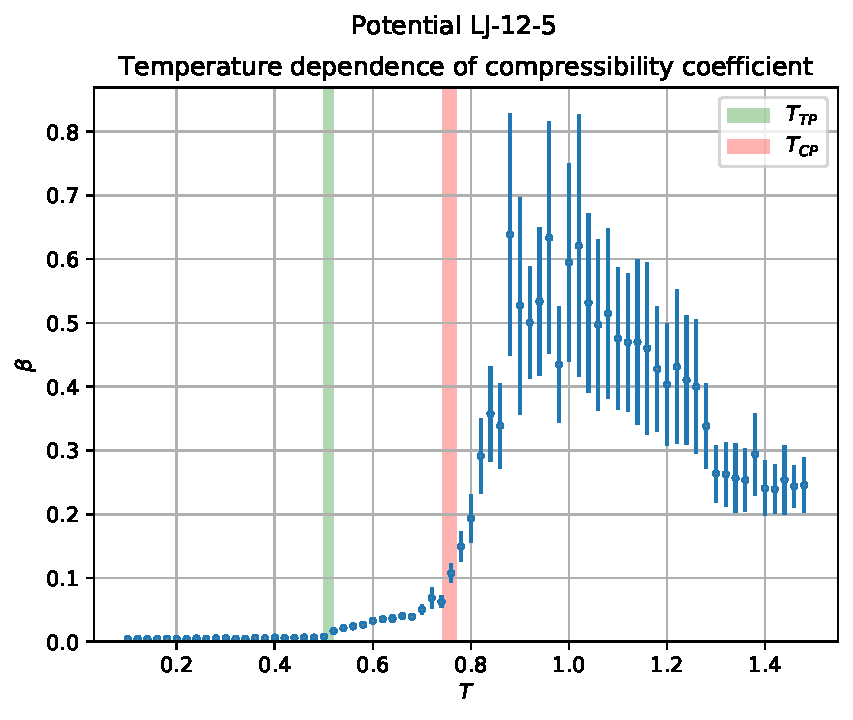
\includegraphics[width=\textwidth, keepaspectratio]{plot_compress_Potential LJ-12-5_1}
\end{minipage}
%\hfill
\begin{minipage}[h]{0.45\linewidth}
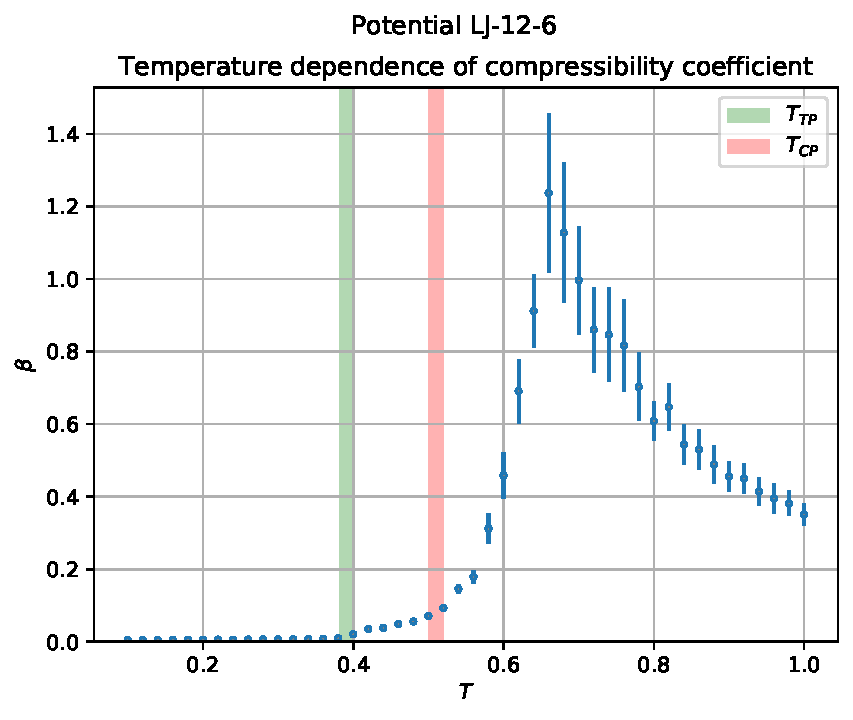
\includegraphics[width=\textwidth, keepaspectratio]{plot_compress_Potential LJ-12-6_1}
\end{minipage}
\caption{Температурная зависимость коэффициента $\beta$, который в мягких взаимодействиях совпадает с сжимаемостью вещества.}
\label{risBeta}
\end{center}
\end{figure}


\begin{figure}[h]
\begin{center}
\begin{minipage}[h]{0.45\linewidth}
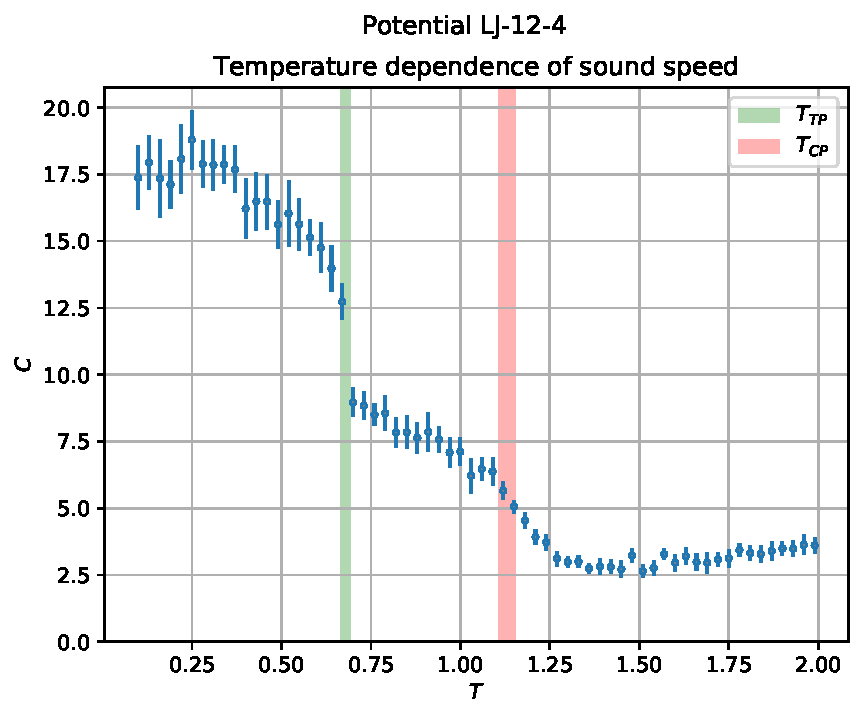
\includegraphics[width=\textwidth, keepaspectratio]{sound_speed_Potential LJ-12-4_1}
\end{minipage}
%\hfill
\begin{minipage}[h]{0.45\linewidth}
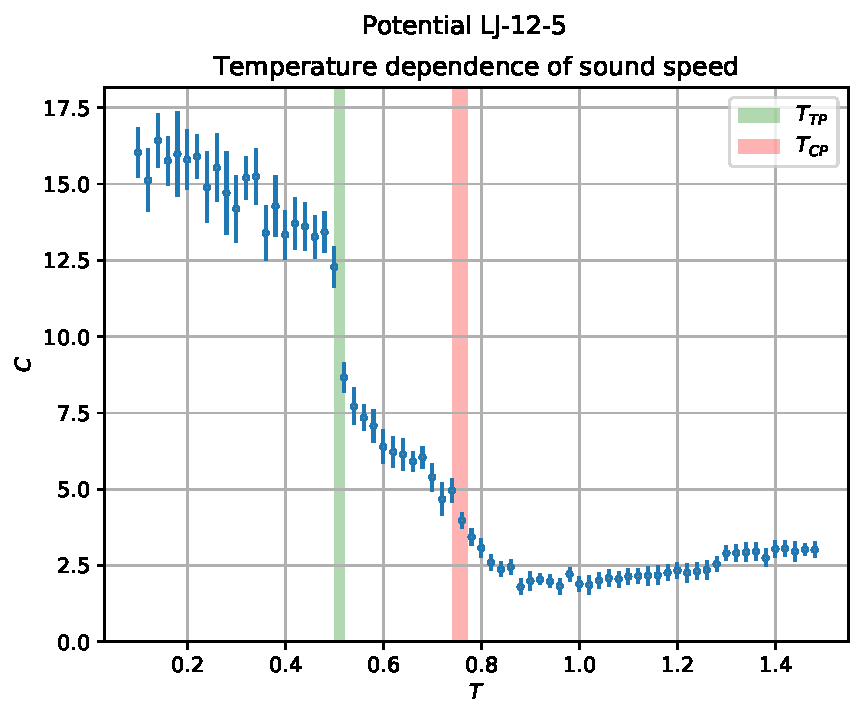
\includegraphics[width=\textwidth, keepaspectratio]{sound_speed_Potential LJ-12-5_1}
\end{minipage}

\begin{minipage}[h]{0.45\linewidth}
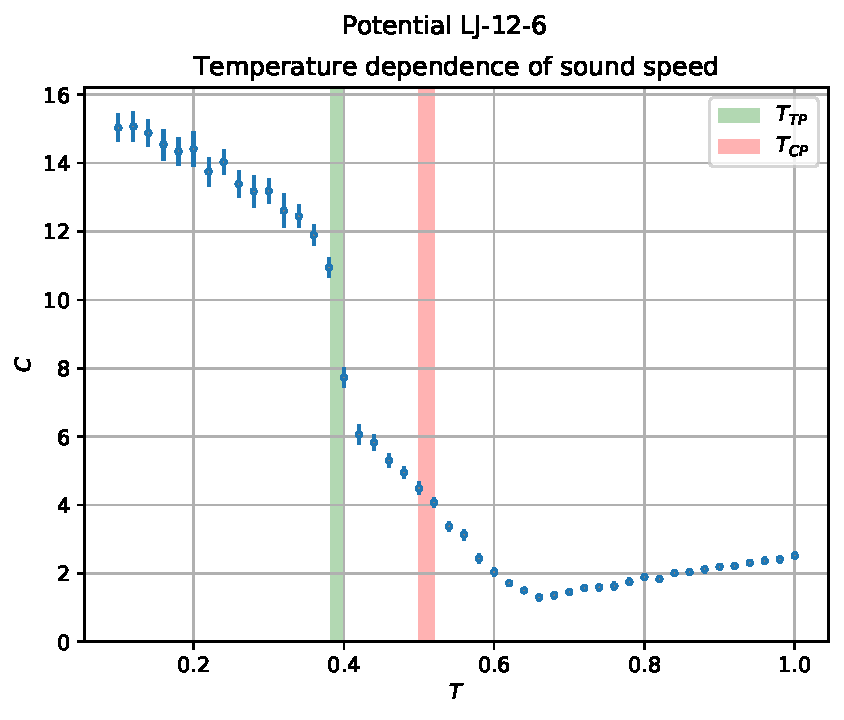
\includegraphics[width=\textwidth, keepaspectratio]{sound_speed_Potential LJ-12-6_1}
\end{minipage}
%\hfill
\begin{minipage}[h]{0.45\linewidth}
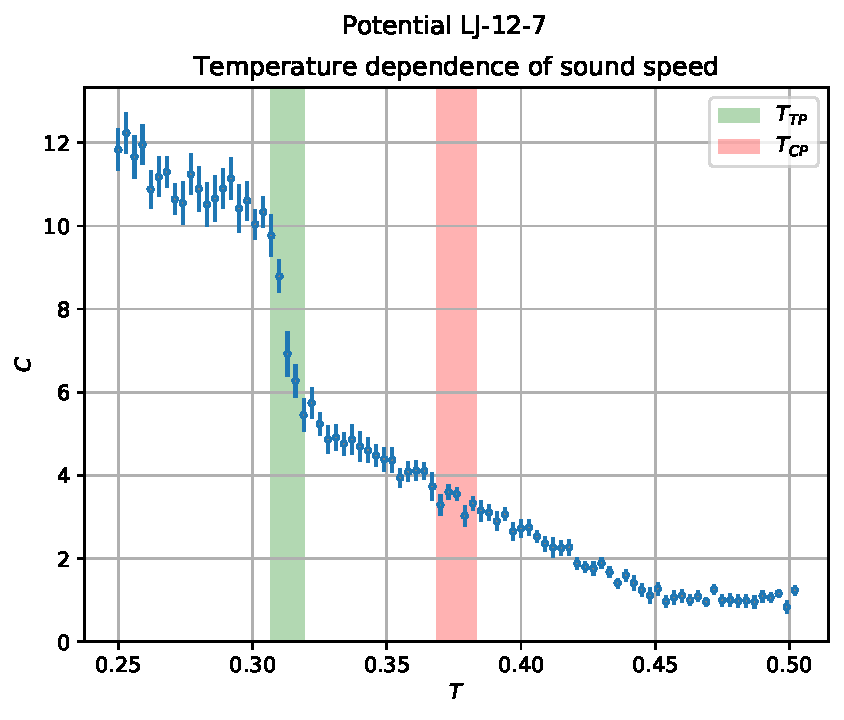
\includegraphics[width=\textwidth, keepaspectratio]{sound_speed_Potential LJ-12-7_1}
\end{minipage}
\caption{Температурная зависимость величины $C$, которая в мягких взаимодействиях совпадает со скоростью звука.}
\label{risC}
\end{center}
\end{figure}

Известно, что зависимость скорости звука вблизи критической точки изменяется по закону:
\begin{equation}
    C \sim v(T_{CP} - T)^{(1-\beta_c)/2},
    \label{eqFitC}
\end{equation}
где $v$ - подгоночный коэффициент.

Аппроксимировав данной зависимостью скорость звука, можно проверить правильность определения критической точки методом, предложенным в разделе \ref{C2_1}.

Однако при численной проверке правильности определения производной $\frac{\partial P}{\partial V}$, выяснилось, что уравнение \ref{eqPv} справедливо только для систем с мягким взаимодействием, например с потенциалом Юкавы. В случае жестких взаимодействий, данное уравнение не удовлетворяет точностью, и дает значения отличающиеся в несколько раз от реальных.

Таким образом, выяснено, что данный подход неприменим в случае жестких взаимодействий, к которым относится потенциал Леннарда-Джонса, и таким образом не получится выяснить точное значение скорости звука и сжимаемости системы данным способом.  

Предположительно, это связано с сильной зависимостью плотности частицы от соседних частиц. Однако в случае успешного нахождения корреляций между локальными флуктуациями плотности и глобальными, эта задача может быть успешно решена, что является перспективным направлением продолжения данной работы.  

Кроме того, интересное поведение проявляют температурные зависимости моментов плотности, изображенные на рисунке \ref{risMu}, которые могут быть непосредственно найдены как для систем с жесткими взаимодействиями, так и с мягкими. 

Данные величины вычисляются по следующей формуле:
\begin{equation}
\mu_i = \mathbb{M} \left[ |\rho - \mathbb{M} \rho|^i \right]
\label{eqMui}
\end{equation}

\begin{figure}[h]
\begin{center}
\begin{minipage}[h]{0.45\linewidth}
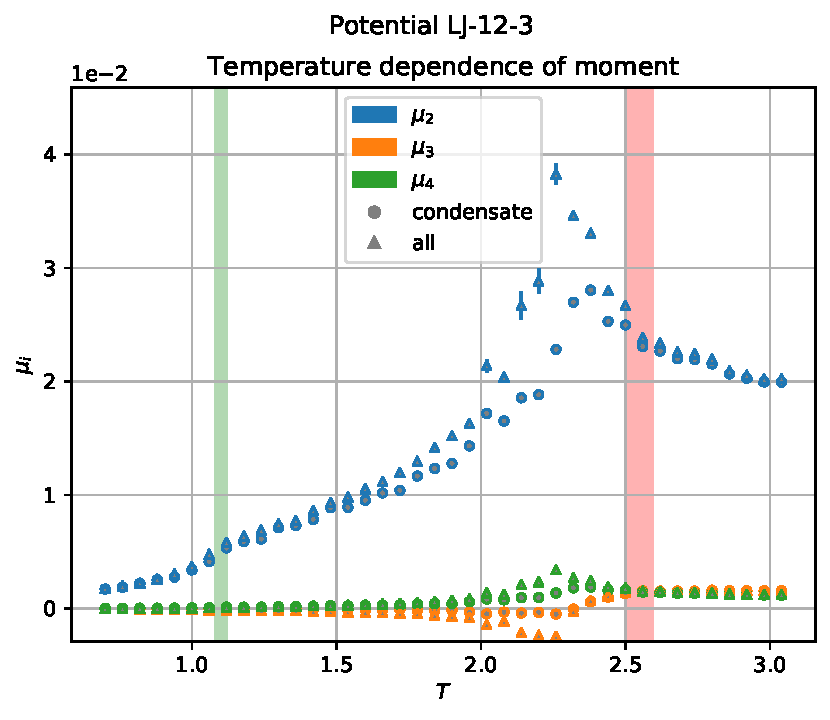
\includegraphics[width=\textwidth, keepaspectratio]{plot_moment_Potential LJ-12-3_1}
\end{minipage}
%\hfill
\begin{minipage}[h]{0.45\linewidth}
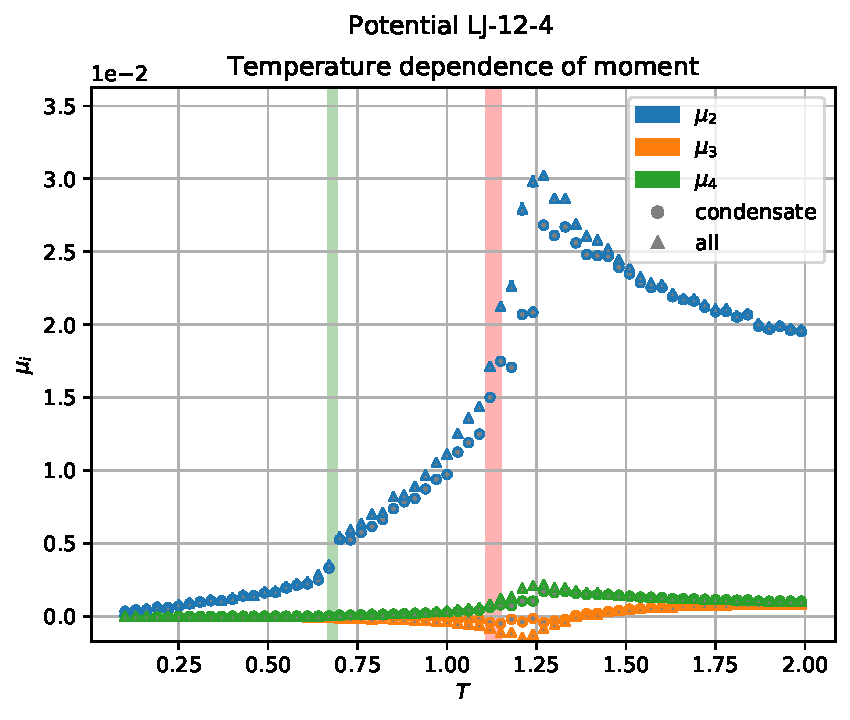
\includegraphics[width=\textwidth, keepaspectratio]{plot_moment_Potential LJ-12-4_1}
\end{minipage}


\begin{minipage}[h]{0.45\linewidth}
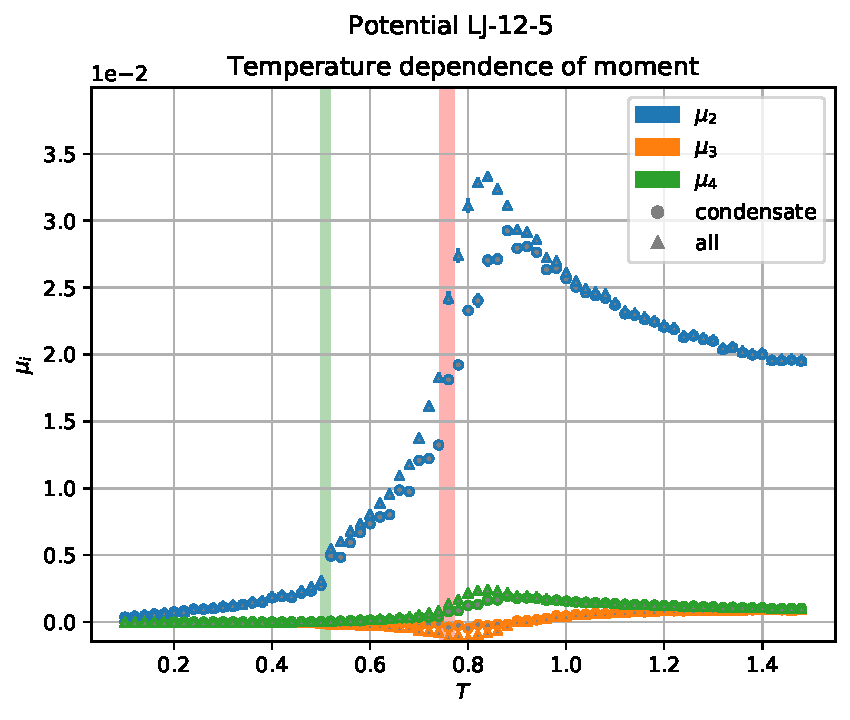
\includegraphics[width=\textwidth, keepaspectratio]{plot_moment_Potential LJ-12-5_1}
\end{minipage}
%\hfill
\begin{minipage}[h]{0.45\linewidth}
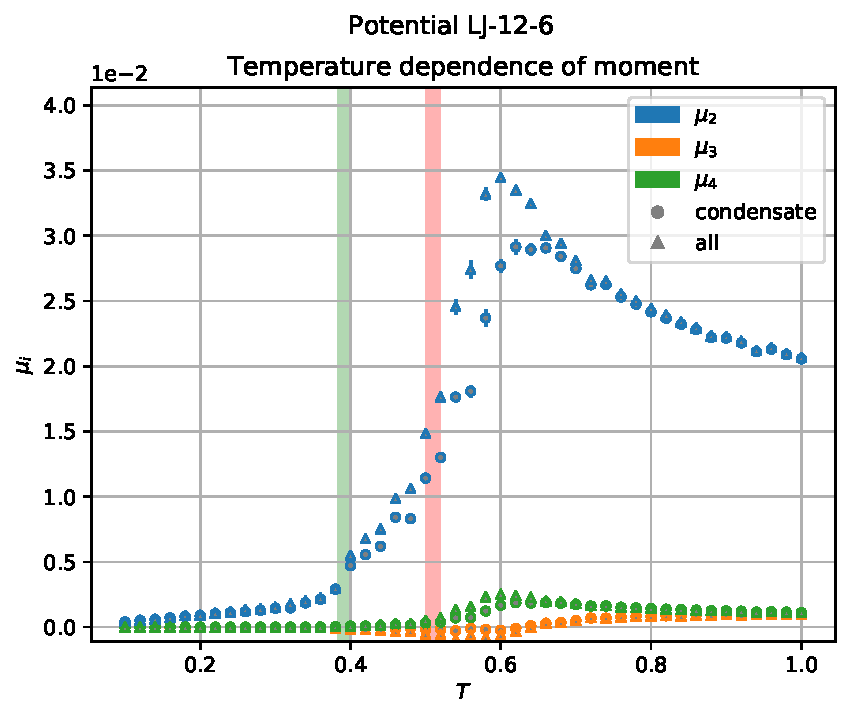
\includegraphics[width=\textwidth, keepaspectratio]{plot_moment_Potential LJ-12-6_1}
\end{minipage}
\caption{Температурная зависимость моментов плотности, в зависимости от потенциала взаимодействия, вычисляемые по формуле \ref{eqMui}.}
\label{risMu}
\end{center}
\end{figure}

По данной зависимости можно судить о температуре с максимальными флуктуациями плотности системы, так называемой линии Видома. Она расположена в окрестности температуры, в которой величина второго момента достигает максимального значения.

\begin{figure}[h]
\begin{center}
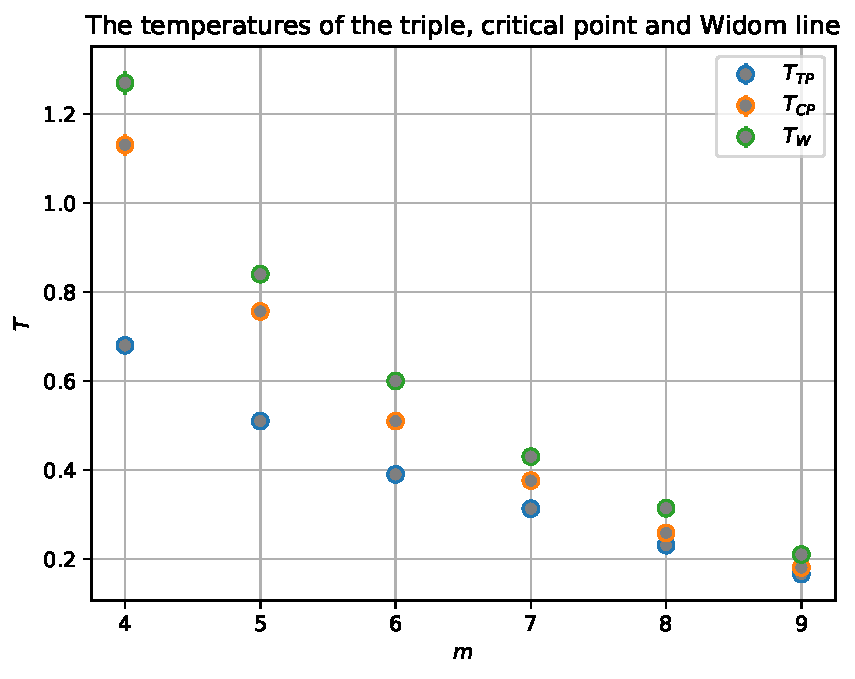
\includegraphics[width=0.7\textwidth]{temperatures_triple_critical_Widom}
\caption{Зависимость тройной, критической точки и линии Видома от дальнодействия притяжения ($m$ в уравнении \ref{eqLJ}). Подробности в основном тексте.}
\label{risTcpTtpWlNoFrac}
\end{center}
\end{figure}

На рисунке \ref{risTcpTtpWlNoFrac} изображены зависимости от дальнодействия притяжения тройной, критической точки и линии Видома.

Как можно заметить, наибольшее влияние значение $m$ оказывает на температуру критической точки, в то время как температура тройной точки изменяется слабее. Предположительно, это связано с тем, что на положение тройной точки большее влияние оказывает отталкивание в системе, в то время как положение критической точки обусловлено дальнодействием, так как позволяет частицам, взаимодействуя на более дальних расстояниях, собираться в капли при критической температуре.

\begin{figure}[h]
\begin{center}
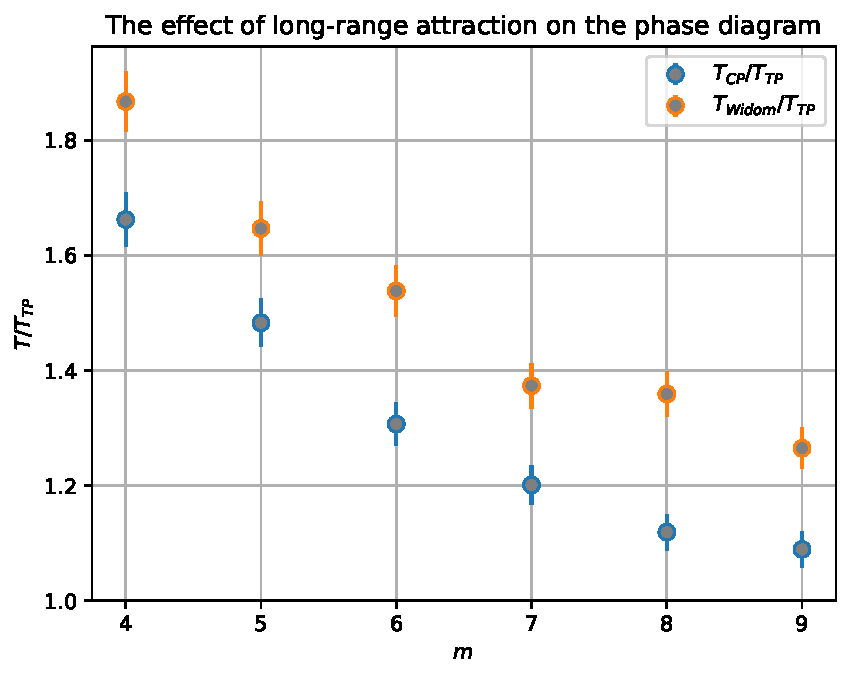
\includegraphics[width=0.7\textwidth]{effect_of_long-range_attraction}
\caption{Зависимость отношения критической точки к тройной, и линии Видома к тройной в зависимости от дальнодействия притяжения ($m$ в уравнении \ref{eqLJ}).}
\label{risTcpTtp}
\end{center}
\end{figure}

Построив отношение температуры линии Видома к тройной точке системы (изображена на рисунке \ref{risTcpTtp}), можно заметить, что ее поведение практически полностью совпадает с поведением критической точки. Из этого можно сделать предположение, что на положение линии Видома, как и на положение критики, большее влияние оказывает слагаемое притяжения, нежели отталкивания, как и на положение критической точки. 

Также, можно предположить, что при некоторых значениях $m$, критическая температура и температура плавления совпадут, и система перейдет в состояние геля. 

Гель -- это структурированная система, состоящая из высокомолекулярных и низкомолекулярных веществ. Наличие трёхмерного полимерного каркаса дает гелям механические свойства твёрдых тел: отсутствие текучести, способность сохранять форму, прочность и способность к деформации (пластичность и упругость).

Таким образом, продемонстрирована возможность изучения с помощью данного метода перехода от обычной молекулярной системы к гелям, а также влияния дальнодействия притяжение на тройную, критическую, и точку максимальных флуктуаций плотности. 

\section{Выводы главы}\label{C2_4}

Таким образом, были рассмотрены методы, которые позволяют определить некоторые термодинамические свойства системы, используя только координаты частиц в системе. Продемонстрирован метод распознавания фаз, позволяющий классифицировать все частицы в системе как газ, поверхность или конденсат, который был существенно модернизирован в рамках данной работы, и в некоторых случаях позволяет существенно улучшить распознавание.

Также в данной главе был рассмотрен способ получения фазовых диаграмм в координатах $\rho, T$, который основан на вычислении математического ожидания плотности конденсата и косвенного определения плотности газа, что является нововведением для данного метода, позволяющим убрать влияние поверхностных частиц на значения плотности газа. 
Был рассмотрен метод получения значений критической точки, с помощью аппроксимации ветвей бинодали, который удалось автоматизировать с помощью составления функции невязки для произвольных критических коэффициентов и температур аппроксимации.
Предложен способ вычислений коэффициента сжимаемости и скорости звука в веществе, используя только статистику распределение плотностей в системе. Так же по данной статистике удалось определить температуру наибольших флуктуаций плотности в системе, что скорее всего соответствует линии Видома.

Результат работы всех этих методов дает возможность выяснить влияние притяжения между частицами на фазовые диаграммы, что позволяет предсказывать термодинамические свойства систем с различными потенциалами взаимодействия. 

\newpage

\newpage
\begin{center}
\textbf{\large ГЛАВА 3 \\ Диффузия от тройной до критической точки}
\end{center}
\refstepcounter{chapter}


% \section*{}
\addcontentsline{toc}{chapter}{ГЛАВА 3. Диффузия от тройной до критической точки}


\section{Изучение диффузии методами молекулярной динамики}\label{C3_1}

Имея координаты всех частиц в системе, можно пронаблюдать за перемещением каждой частицей в отдельности и оценить коэффициент диффузии и другие параметры переноса в данной системе.

На рисунке \ref{risTreck} изображены траектории частиц в исследуемой системе на примере потенциала Леннарда--Джонса при различной температуре.  Для демонстрации динамики системы были взяты первые 10 кадров, используемые в статистике, описанной в разделе \ref{C2_2}, с шагом по времени между кадрами равными $0.5\tau$. Траектории раскрашены в зависимости от перемещения частицы за 10 кадров наблюдения. Частицам, практически не поменявшим свое расположение соответствует темно-синий цвет. В данном случае наиболее оптимальным было считать максимальным перемещением $3\sigma$, где $\sigma$ - безразмерная единица измерения длинны в моделировании, равная единице.

Как можно заметить, частицы, распознанные как конденсат в разделе \ref{C2_2}, демонстрируют меньшие длинны траектории чем газ, что свидетельствует о достаточно хорошей точности распознавания фаз, описанной в разделе \ref{C2_1}. 

\begin{figure}[h]
\begin{center}
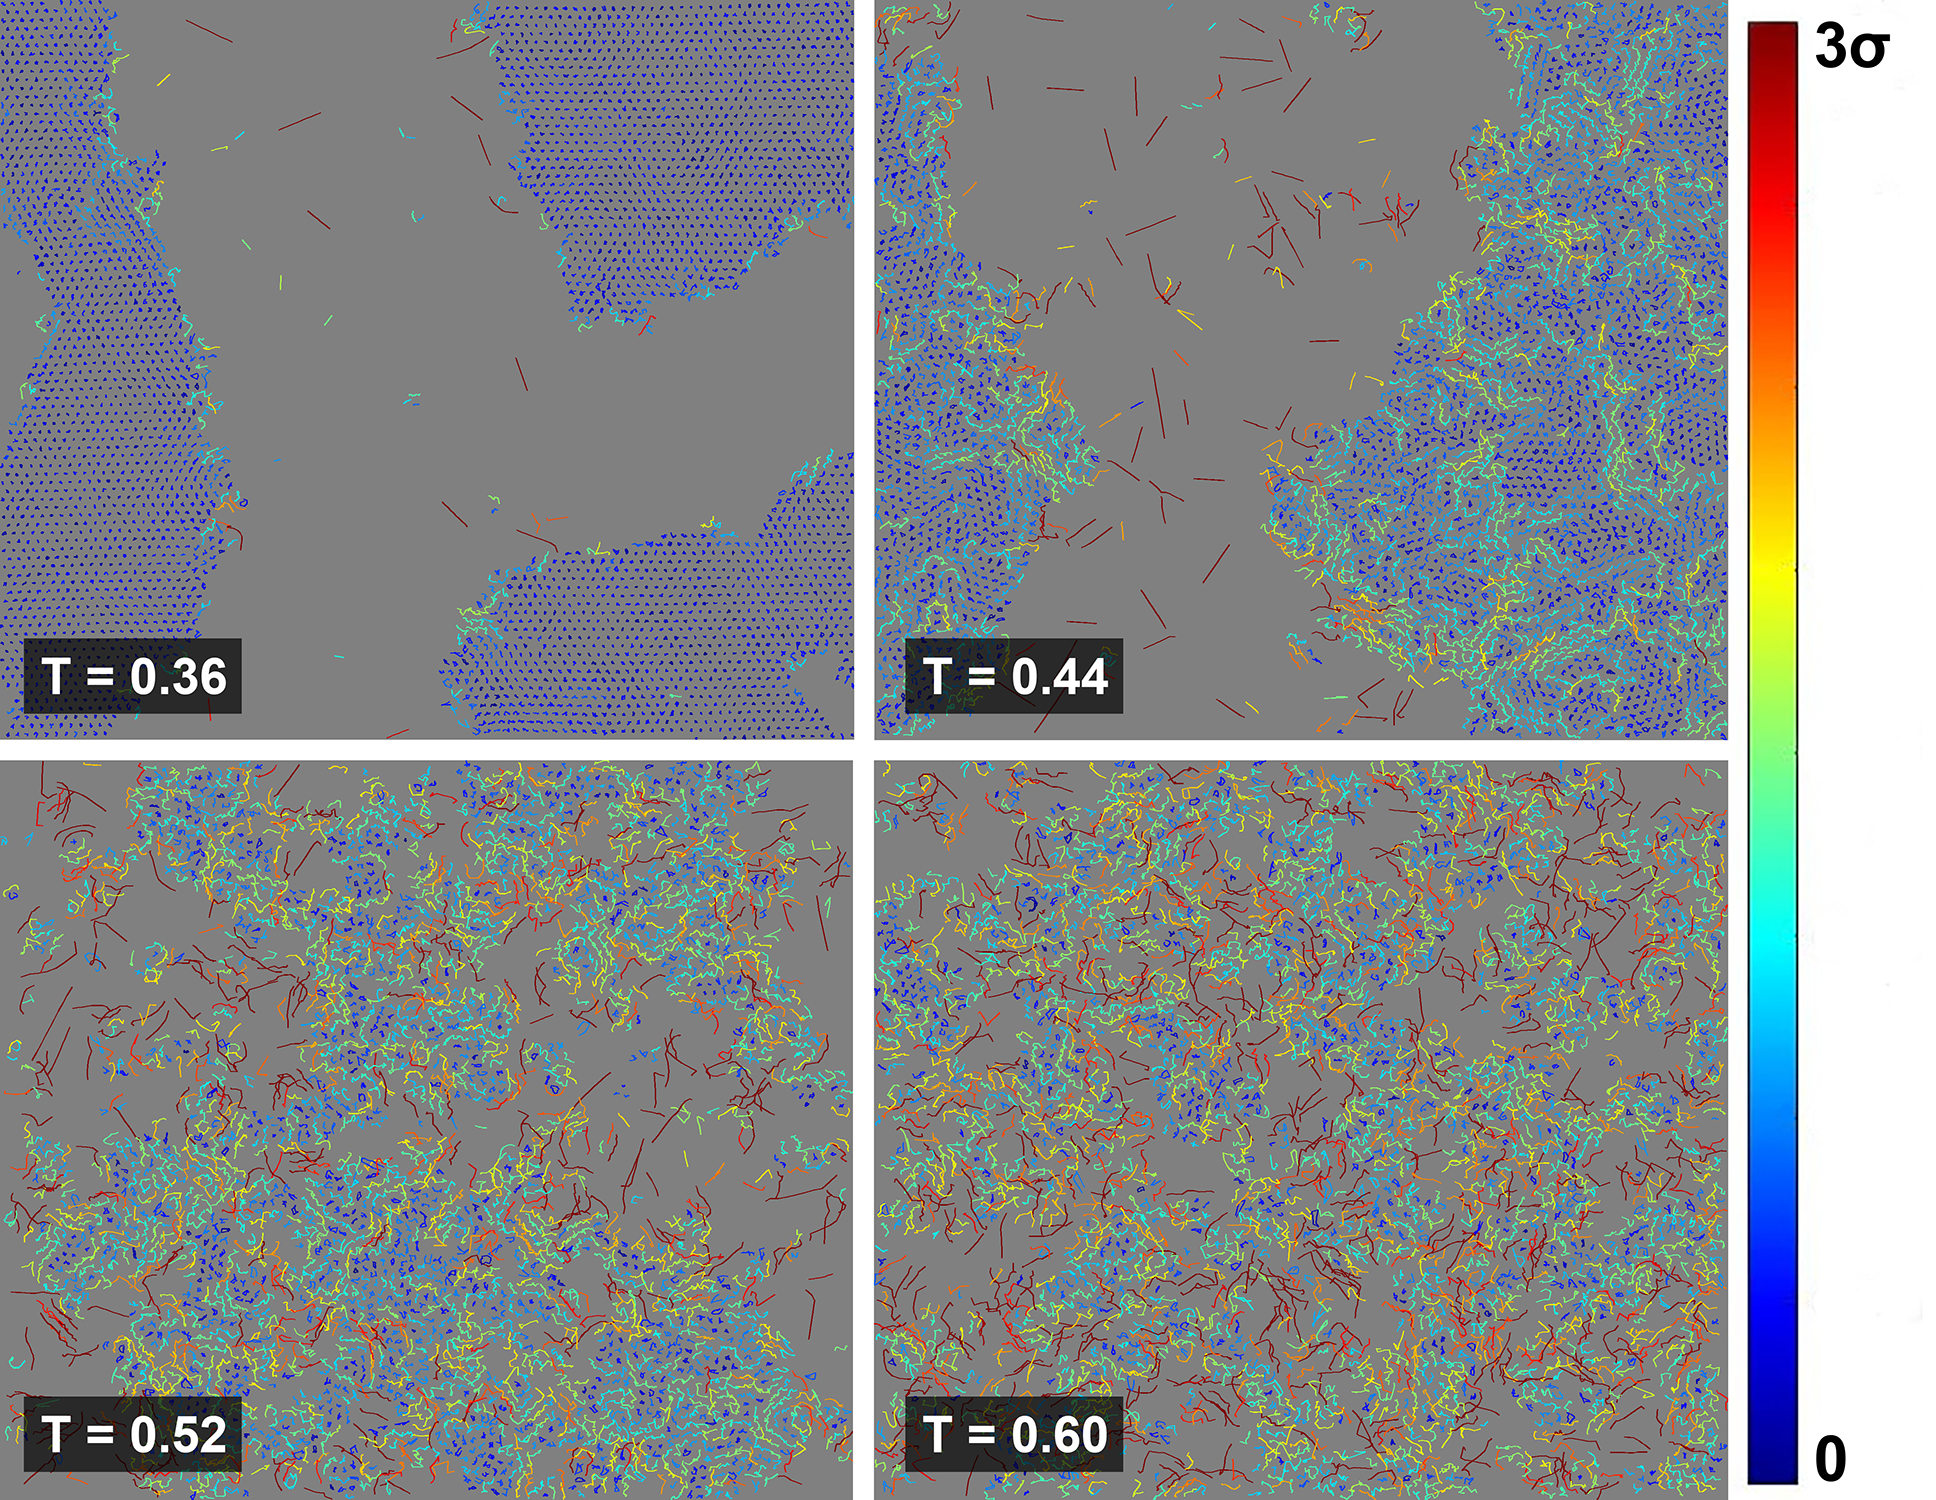
\includegraphics[width=0.7\textwidth]{Diffusion}
\caption{Смещение частиц от начального положения за 10 кадров моделирования. Цветом показана величина смещения в $\sigma$ (единица измерения длинны). Наиболее подвижным частицам соответствует темно-красный цвет траектории.}
\label{risTreck}
\end{center}
\end{figure}

Количество частиц на кадре в общем случае может быть не одинаковым. В реальных экспериментах с коллоидными суспензиями это обусловлено смещением частиц за пределы кадра, или потерей частицы на кадре из-за неидеальности распознавания объектов на изображении используемым методом. В случае моделирования причинами непостоянства количества частиц могут быть смещение частицы за пределы исследуемой области, либо отсева частиц с бесконечными гранями ячейки вороного, расположенной на периферии, для которой не удается определить ни соседей, ни площади. Такие частицы не участвуют в статистике ни расчета термодинамических параметров во второй главе, ни в расчете параметров переноса. 

Зная смещения всех частиц от их изначального положения в системе, с $t = 0$, можно рассчитать среднеквадратичное смещение частиц с помощью уравнения:
\begin{equation}
    \sigma^2(t) = \sum\limits_{\alpha = 1}^{N(t)} (r_{\alpha}(t) - r_{\alpha}(0))^2 / N(t),
    \label{eqRMS}
\end{equation}
где $\sigma^2(t)$ - среднеквадратичное смещение частиц, $N(t)$ - количество частиц в данный момент времени в кадре, $r_{\alpha}(t)$ - положение частицы в момент времени $t$, $r_{\alpha}(0)$ - положение частицы в начальный момент времени $t = 0$.

\begin{figure}[h]
\begin{center}
\begin{minipage}[h]{0.45\linewidth}
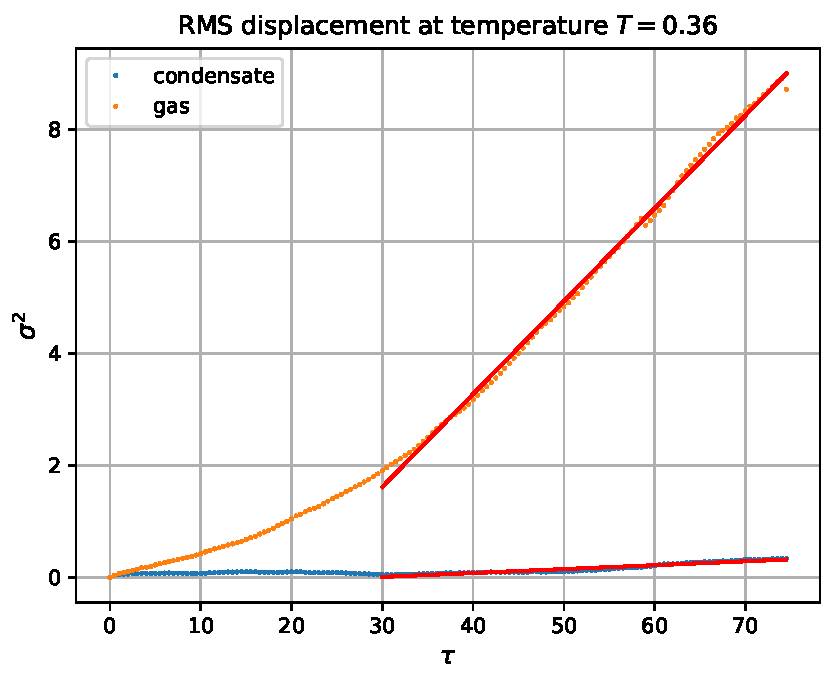
\includegraphics[width=\textwidth, keepaspectratio]{diffusion_fit_0.36}
\end{minipage}
%\hfill
\begin{minipage}[h]{0.45\linewidth}
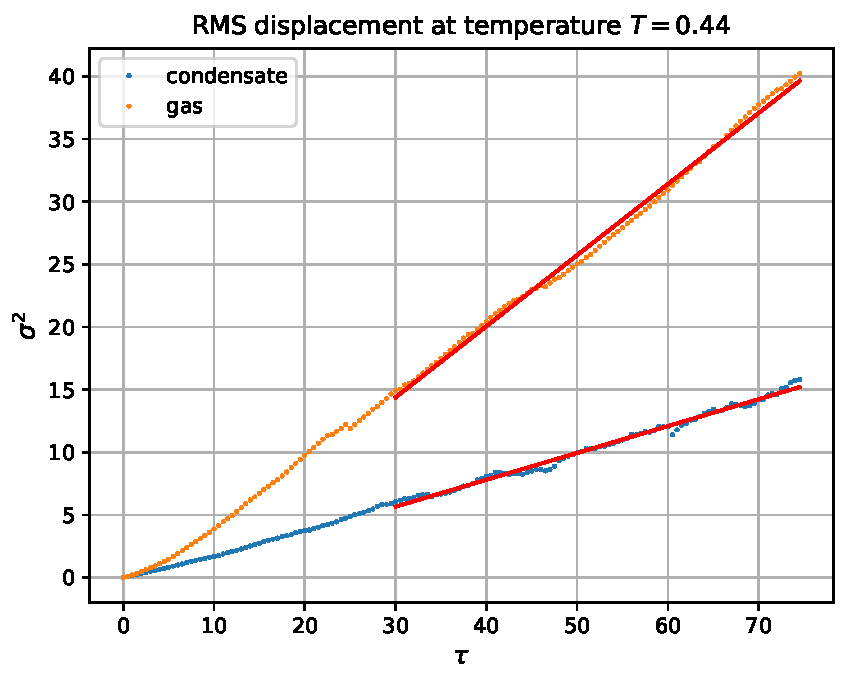
\includegraphics[width=\textwidth, keepaspectratio]{diffusion_fit_0.44}
\end{minipage}

\begin{minipage}[h]{0.45\linewidth}
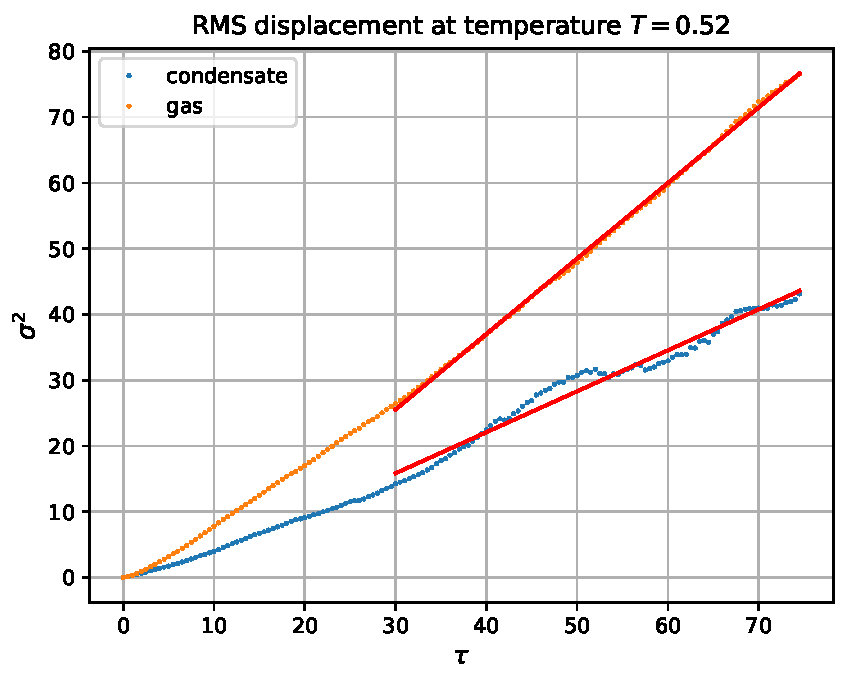
\includegraphics[width=\textwidth, keepaspectratio]{diffusion_fit_0.52}
\end{minipage}
%\hfill
\begin{minipage}[h]{0.45\linewidth}
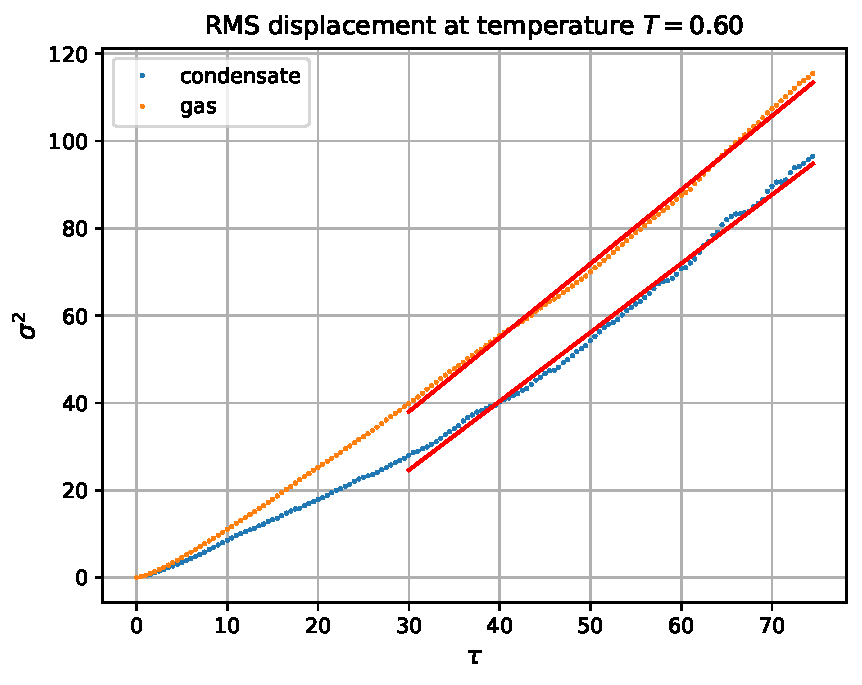
\includegraphics[width=\textwidth, keepaspectratio]{diffusion_fit_0.60}
\end{minipage}
\caption{Временная зависимость среднеквадратичного смещения частиц для различных температур на примере потенциала Леннарда-Джонса. Синим цветом обозначено среднеквадратичное смещение конденсированных частиц,  а оранжевым - всех частиц в исследуемой системе.}
\label{risRMS}
\end{center}
\end{figure}

График зависимости среднеквадратичного смещения для подсистем конденсированных частиц и всех (все частицы в системе, включая газовые и конденсат) от безразмерного времени для различных температур изображен на рисунке \ref{risRMS}.

Так как для двумерной системы верно равенство $\sigma^2(t) = 4Dt$, то коэффициент диффузии выражается следующей формулой:
\begin{equation}
    D = \frac{\sigma^2(t)}{4t},
    \label{eqD}
\end{equation}
где $D$ - коэффициент диффузии в веществе.

Его можно получить путем аппроксимации среднеквадратичного смещения функцией $\sigma^2(t) = 4Dt + a$, где $a$ - подгоночный коэффициент. Подгоночный коэффициент $a$ появляется в следствие того, что аппроксимация производится начиная не с 0 по времени, а с некоторого значения, когда функция становится линейной. Данный эффект хорошо наблюдается при $T = 0.36$ на рисунке \ref{risRMS}. Он возникает по причине большого свободного пробега частиц, при котором частицы движутся свободно, что соответствует параболической форме траектории. Экспериментально установлено, что для данных экспериментов достаточно использовать последние $60\%$ точек, для правильной аппроксимации. 
На рисунке \ref{risRMS} она показана сплошной красной линией, которая аппроксимирует среднеквадратичное смещение с достаточно хорошей точностью.

\begin{figure}[h]
\begin{center}
\begin{minipage}[h]{0.45\linewidth}
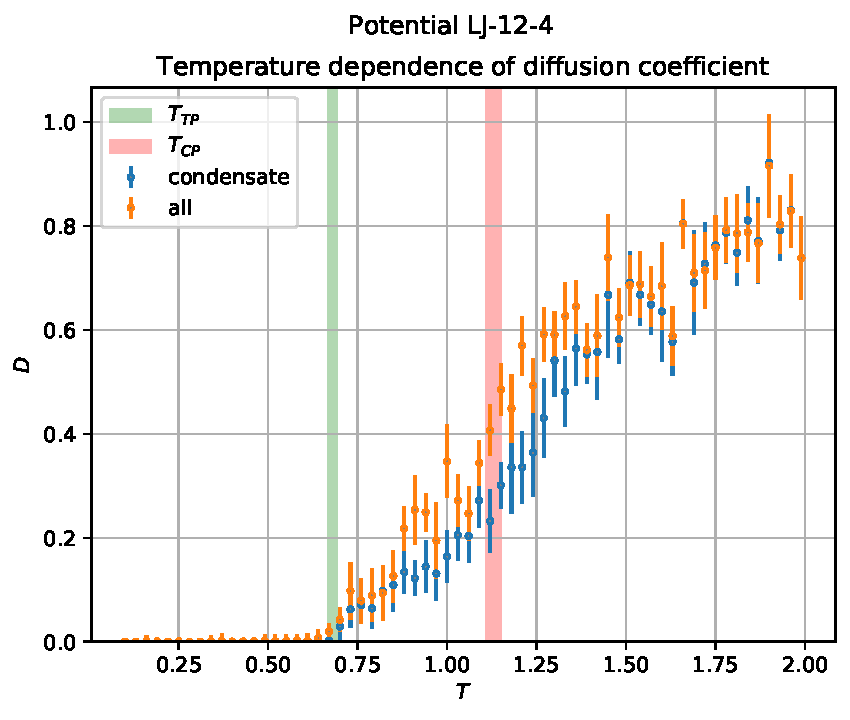
\includegraphics[width=\textwidth, keepaspectratio]{plot_diffusion_Potential LJ-12-4_1}
\end{minipage}
\begin{minipage}[h]{0.45\linewidth}
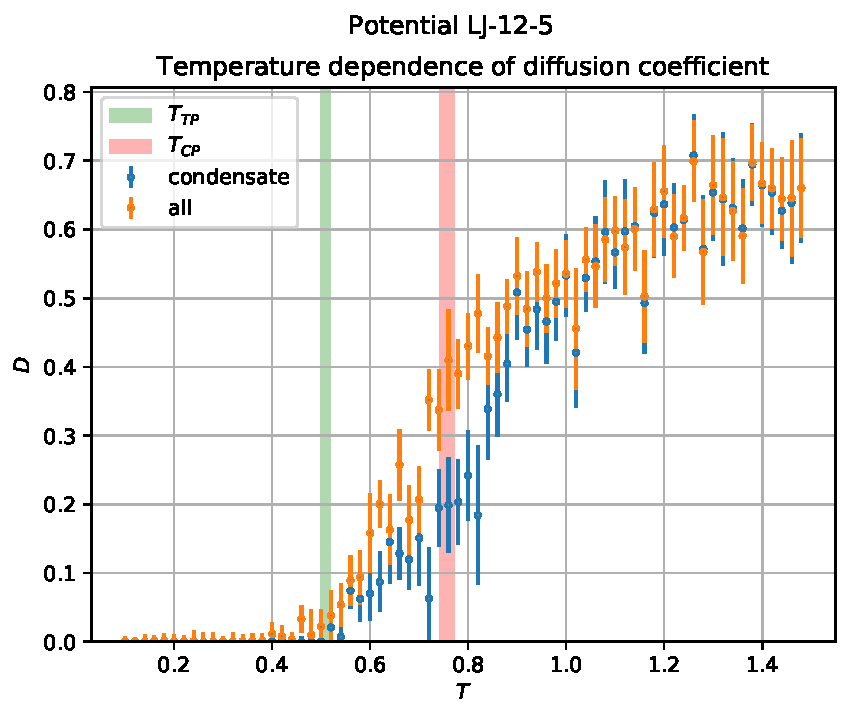
\includegraphics[width=\textwidth, keepaspectratio]{plot_diffusion_Potential LJ-12-5_1}
\end{minipage}
\begin{minipage}[h]{0.45\linewidth}
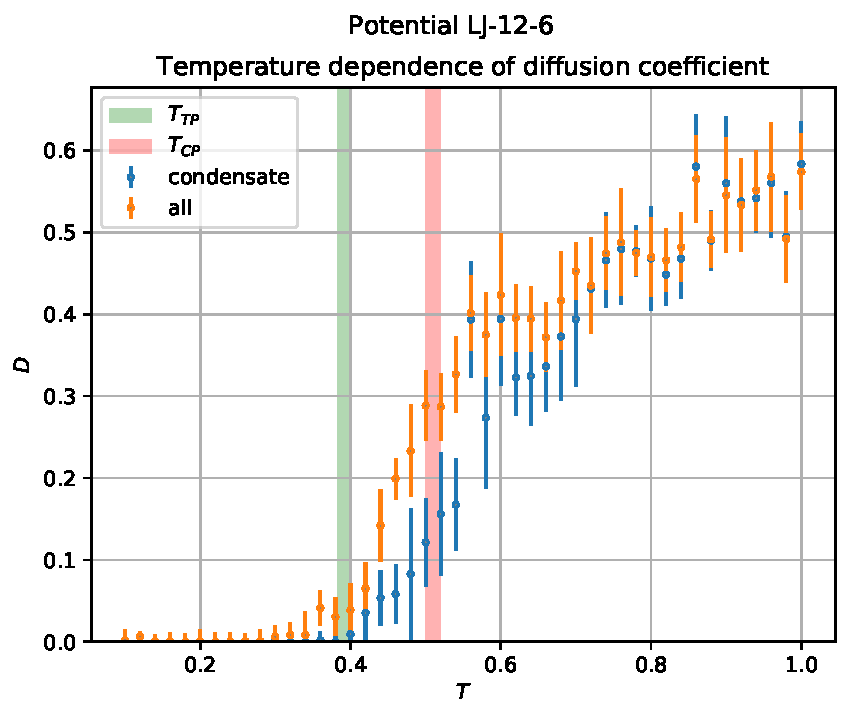
\includegraphics[width=\textwidth, keepaspectratio]{plot_diffusion_Potential LJ-12-6_1}
\end{minipage}
\begin{minipage}[h]{0.45\linewidth}
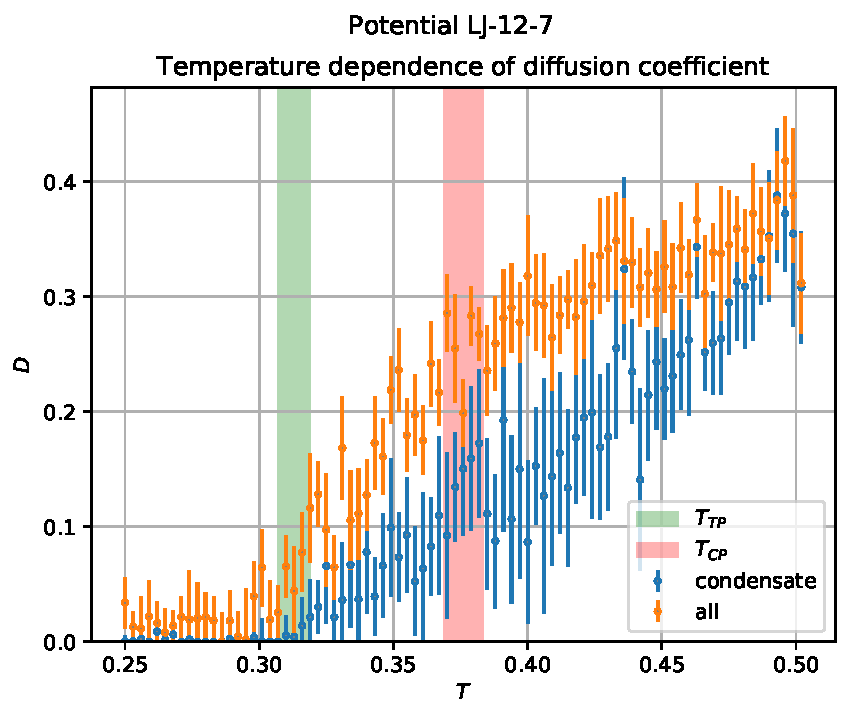
\includegraphics[width=\textwidth, keepaspectratio]{plot_diffusion_Potential LJ-12-7_1}
\end{minipage}
\caption{Температурная зависимость коэффициента диффузии для различных потенциалов взаимодействия. Синим цветом обозначена диффузия в конденсате, желтым -- во всей системе.}
\label{risD}
\end{center}
\end{figure}

Проводя данные вычисления для различных температур, можно установить температурную зависимость коэффициента диффузии для различных потенциалов взаимодействия, изображенную на рисунке \ref{risD}.

Полученные результаты хорошо согласуются с экспериментом, например в $LJ12-6$ температура плавления $T_{TP} = 0.405$, что соответствует температуре, при которой значение коэффициента диффузии начинает расти.

Коэффициент диффузии, рассчитанный таким образом, может быть использован для определения тройной точки, так как однозначно при различных потенциалах показывает резкий рост смещения частиц относительно своих изначальных положений, что характерно при плавлении веществ.

\begin{figure}[h]
\begin{center}
\begin{minipage}[h]{0.45\linewidth}
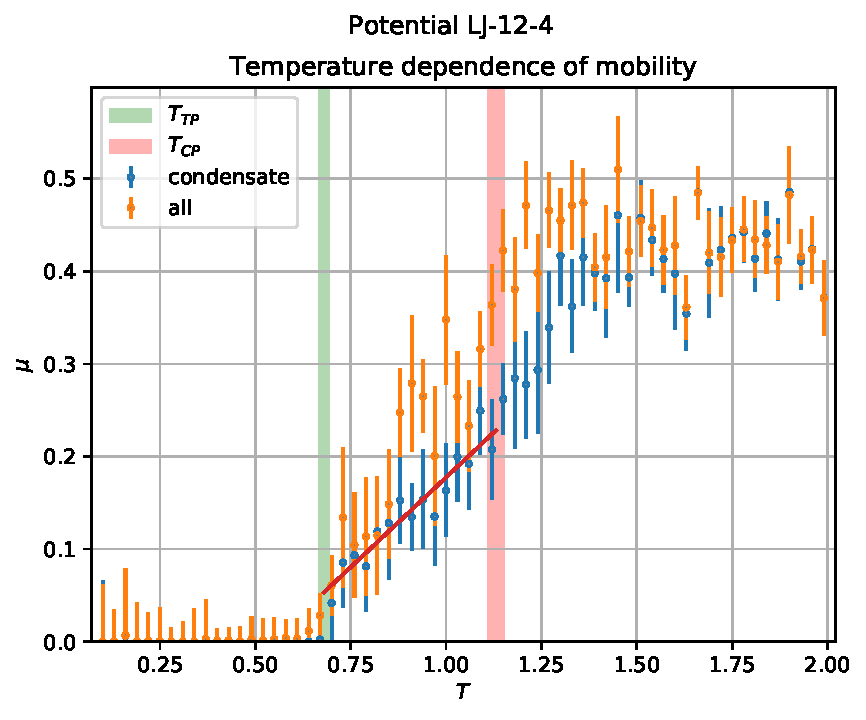
\includegraphics[width=\textwidth, keepaspectratio]{plot_mobility_Potential LJ-12-4_1}
\end{minipage}
%\hfill
\begin{minipage}[h]{0.45\linewidth}
\includegraphics[width=\textwidth, keepaspectratio]{plot_mobility_Potential LJ-12-5_1}
\end{minipage}
\begin{minipage}[h]{0.45\linewidth}
\includegraphics[width=\textwidth, keepaspectratio]{plot_mobility_Potential LJ-12-6_1}
\end{minipage}
%\hfill
\begin{minipage}[h]{0.45\linewidth}
\includegraphics[width=\textwidth, keepaspectratio]{plot_mobility_Potential LJ-12-7_1}
\end{minipage}
\caption{Температурная зависимость подвижности для различных потенциалов взаимодействия. Синим цветом обозначена подвижность в конденсате, желтым -- во всей системе.}
\label{risMuDiff}
\end{center}
\end{figure}

Кроме диффузии мы можем вычислить подвижность частиц в системе, которая определяется следующим образом:
\begin{equation}
    \mu  = \frac{D}{T},
    \label{eqMuDiff}
\end{equation}
где $\mu$ - подвижность частиц.

Зависимость подвижности частиц от температуры представлена на рисунке \ref{risMuDiff}.
Как можно заметить, данная зависимость практически линейна в промежутке от тройной до критической точки. Аппроксимация подвижности частиц в пределах жидкой фазы позволяет выяснить температурное влияние на изменение подвижности, в зависимости от дальнодействия притяжения.

\begin{figure}[h]
\begin{center}
\includegraphics[width=\textwidth]{mobility_fitting_factors}
\caption{График зависимости параметров аппроксимации подвижности от тройной до критической точки линейной функцией.}
\label{risDmu}
\end{center}
\end{figure}

На рисунке \ref{risDmu} представлена зависимость параметров аппроксимации подвижности конденсированных частиц от тройной до критической точки линейной функцией. Физический смыл у данных коэффициентов следующий, $b$ - значение подвижности частиц в тройной точке, а $k$ - производная значения подвижности по температуре. 

Анализируя зависимость подвижности в тройной точке, можно предположить, что ее уменьшение связано с уменьшением ширины потенциальной ямы, в которой находится частица. В то же время отклик системы на повышение температуры, которым является параметр $k$, повышается. Это может быть связано с уменьшением потенциальной ямы, в которой находится частицы, что позволяет ей легче передвигаться и из нее выходить.

В случае дальнейшего уменьшения дальнодействия в системе, можно будет наблюдать переход вещества в состояние геля, для которого характерно очень сильное влияние температуры на подвижность частиц.


% \section{Связь термодинамических параметров и параметров переноса вещества}\label{C3_2}

% В попытках выяснить зависимость параметров переноса вещества от его термодинамических параметров, были построены зависимости мобильности от сжимаемости и диффузии (рисунки \ref{risMuBeta}, \ref{risDBeta}), а так же зависимость скорости звука от подвижности частиц (рисунок \ref{risCMu}).

% \begin{figure}[h]
% \begin{center}
% \begin{minipage}[h]{0.45\linewidth}
% \includegraphics[width=\textwidth, keepaspectratio]{plot_compress_mobility_Potential LJ-12-4_1}
% \end{minipage}
% %\hfill
% \begin{minipage}[h]{0.45\linewidth}
% \includegraphics[width=\textwidth, keepaspectratio]{plot_compress_mobility_Potential LJ-12-5_1}
% \end{minipage}

% \begin{minipage}[h]{0.45\linewidth}
% \includegraphics[width=\textwidth, keepaspectratio]{plot_compress_mobility_Potential LJ-12-6_1}
% \end{minipage}
% %\hfill
% \begin{minipage}[h]{0.45\linewidth}
% \includegraphics[width=\textwidth, keepaspectratio]{plot_compress_mobility_Potential LJ-12-7_1}
% \end{minipage}
% \caption{Зависимость подвижности от сжимаемости для различных потенциалов взаимодействия. Синим цветом обозначены точки, в которых система принадлежит кристаллической фазе, желтым - жидкой, красным - сверхкритической жидкости.}
% \label{risMuBeta}
% \end{center}
% \end{figure}


% \begin{figure}[h]
% \begin{center}
% \begin{minipage}[h]{0.45\linewidth}
% \includegraphics[width=\textwidth, keepaspectratio]{plot_diffusion_compress_Potential LJ-12-4_1}
% \end{minipage}
% %\hfill
% \begin{minipage}[h]{0.45\linewidth}
% \includegraphics[width=\textwidth, keepaspectratio]{plot_diffusion_compress_Potential LJ-12-5_1}
% \end{minipage}

% \begin{minipage}[h]{0.45\linewidth}
% \includegraphics[width=\textwidth, keepaspectratio]{plot_diffusion_compress_Potential LJ-12-6_1}
% \end{minipage}
% %\hfill
% \begin{minipage}[h]{0.45\linewidth}
% \includegraphics[width=\textwidth, keepaspectratio]{plot_diffusion_compress_Potential LJ-12-7_1}
% \end{minipage}
% \caption{Зависимость диффузии от сжимаемости при различных потенциалах взаимодействия. Синим цветом обозначены точки, в которых система принадлежит кристаллической фазе, желтым - жидкой, красным - сверхкритической жидкости.}
% \label{risDBeta}
% \end{center}
% \end{figure}



% \begin{figure}[h]
% \begin{center}
% \begin{minipage}[h]{0.45\linewidth}
% \includegraphics[width=\textwidth, keepaspectratio]{sound_speed_mobility_Potential LJ-12-4_1}
% \end{minipage}
% %\hfill
% \begin{minipage}[h]{0.45\linewidth}
% \includegraphics[width=\textwidth, keepaspectratio]{sound_speed_mobility_Potential LJ-12-5_1}
% \end{minipage}

% \begin{minipage}[h]{0.45\linewidth}
% \includegraphics[width=\textwidth, keepaspectratio]{sound_speed_mobility_Potential LJ-12-6_1}
% \end{minipage}
% %\hfill
% \begin{minipage}[h]{0.45\linewidth}
% \includegraphics[width=\textwidth, keepaspectratio]{sound_speed_mobility_Potential LJ-12-7_1}
% \end{minipage}
% \caption{Зависимость скорости звука от подвижности при различных потенциалах. Синим цветом обозначены точки, в которых система принадлежит кристаллической фазе, желтым - жидкой, красным - сверхкритической жидкости.}
% \label{risCMu}
% \end{center}
% \end{figure}

% На примере рисунка \ref{risCMu} видно, что по совокупности параметров скорости звука и подвижности частиц система отчетливо делится на три класса, кристаллической, жидкой, и закритической фазе. 

% Такое четкое различие в расположениях точек дает возможность использовать различные классификаторы, например нейронные сети для определения принадлежности определенных точек к той или иной фазе. 


\section{Выводы главы}\label{C3_3}

В данной главе были рассмотрены расчеты диффузии методами молекулярной динамики, и его особенности. Данный метод, в совокупности с методом распознавания фаз, описанном в разделе \ref{C2_1}, позволяет достаточно точно определить подвижность частиц в конденсированной фазе, а так же ее температурную зависимость.

Выявлено влияние изменения температуры на подвижность частиц, в зависимости от дальнодействия притяжения.

% Предложен метод классификации системы на конденсат, жидкость и сверхкритическую жидкость с использованием нейронных сетей.

\newpage
\newpage
\begin{center}
\textbf{\large ЗАКЛЮЧЕНИЕ}
\end{center}
\refstepcounter{chapter}


% \section*{}
\addcontentsline{toc}{chapter}{ЗАКЛЮЧЕНИЕ}
Основные результаты бакалаврской квалификационной работы:
\begin{enumerate}
    \item В работе продемонстрированная актуальность метода изучения молекулярных систем с использованием построения диаграммы Вороного, который, используя только координаты частиц в разные моменты времени, позволяет узнать некоторые термодинамические параметры и параметры переноса в веществе.
    \item Проведена модернизация алгоритма классификации частиц на фазы, которая позволяет улучшить качество классификации и убрать артефакты из статистики распределения плотности частиц.
    \item Проведены серии моделирований обобщенного потенциала взаимодействия Леннарда--Джонса с различным дальнодействием притяжения для определения его роли в расположении критических, тройных точек и линий Видома на фазовых диаграммах вещества. 
    \item Реализован программный пакет для изучения диффузии с разрешением отдельных частиц, и с его помощью установлена роль дальнодействия притяжения на подвижность в веществе. 
\end{enumerate}

% В данной работе рассмотрены методы изучения молекулярных систем, которые, используя только координаты частиц в разные моменты времени, позволяют узнать некоторые термодинамические параметры системы.

% Было показано, каким образом можно эффективно классифицировать частицы на газ, конденсат и поверхность, с помощью разбиение системы на ячейки вороного. Проведена модернизация алгоритма классификации, которая позволяет улучшить качество распознавания фаз, и убрать артефакты из статистики распределения плотности частиц.

% Разработан и автоматизирован метод, позволяющий определять критические точки в веществе с удовлетворительной точностью.

% Установлена роль притяжения в расположении тройных и критических точек, а также точек с наибольшими флуктуациями плотности в системе.

% Предложен способ определения сжимаемости и скорости звука в веществе, используя только распределение плотностей ячеек вороного, а так же способ определения линии Видома для плотности, с помощью моментов величины плотности вещества.

% Установлено влияние дальнодействия притяжения на параметры переноса частиц в веществе, и их температурные зависимости. 
% Предложен способ классификации системы на кристалл, жидкость и сверхкритическую жидкость с помощью нейронных сетей, по параметрам скорости звука и мобильности в веществе.

\newpage

%\bibliographystyle{unsrt}
\bibliographystyle{biblio/gost2008n}
\renewcommand\bibname{\normalsize СПИСОК ИСПОЛЬЗОВАННЫХ ИСТОЧНИКОВ}
\let\BibEmph=\emph
%\bibliographystyle{ugost2008}  %% стилевой файл для оформления по ГОСТу
\bibliography{biblio/biblio}

\end{document}
